
%---------------------------------------------------------------------
\begin{frame}{}
    \begin{center}
    \Large \textcolor{maroon}{Last week}
    \end{center}

\end{frame}
%---------------------------------------------------------------------
%---------------------------------------------------------------------
\begin{frame}{The U.S. healthcare system}
    \vspace{-7mm}
    \begin{center}
        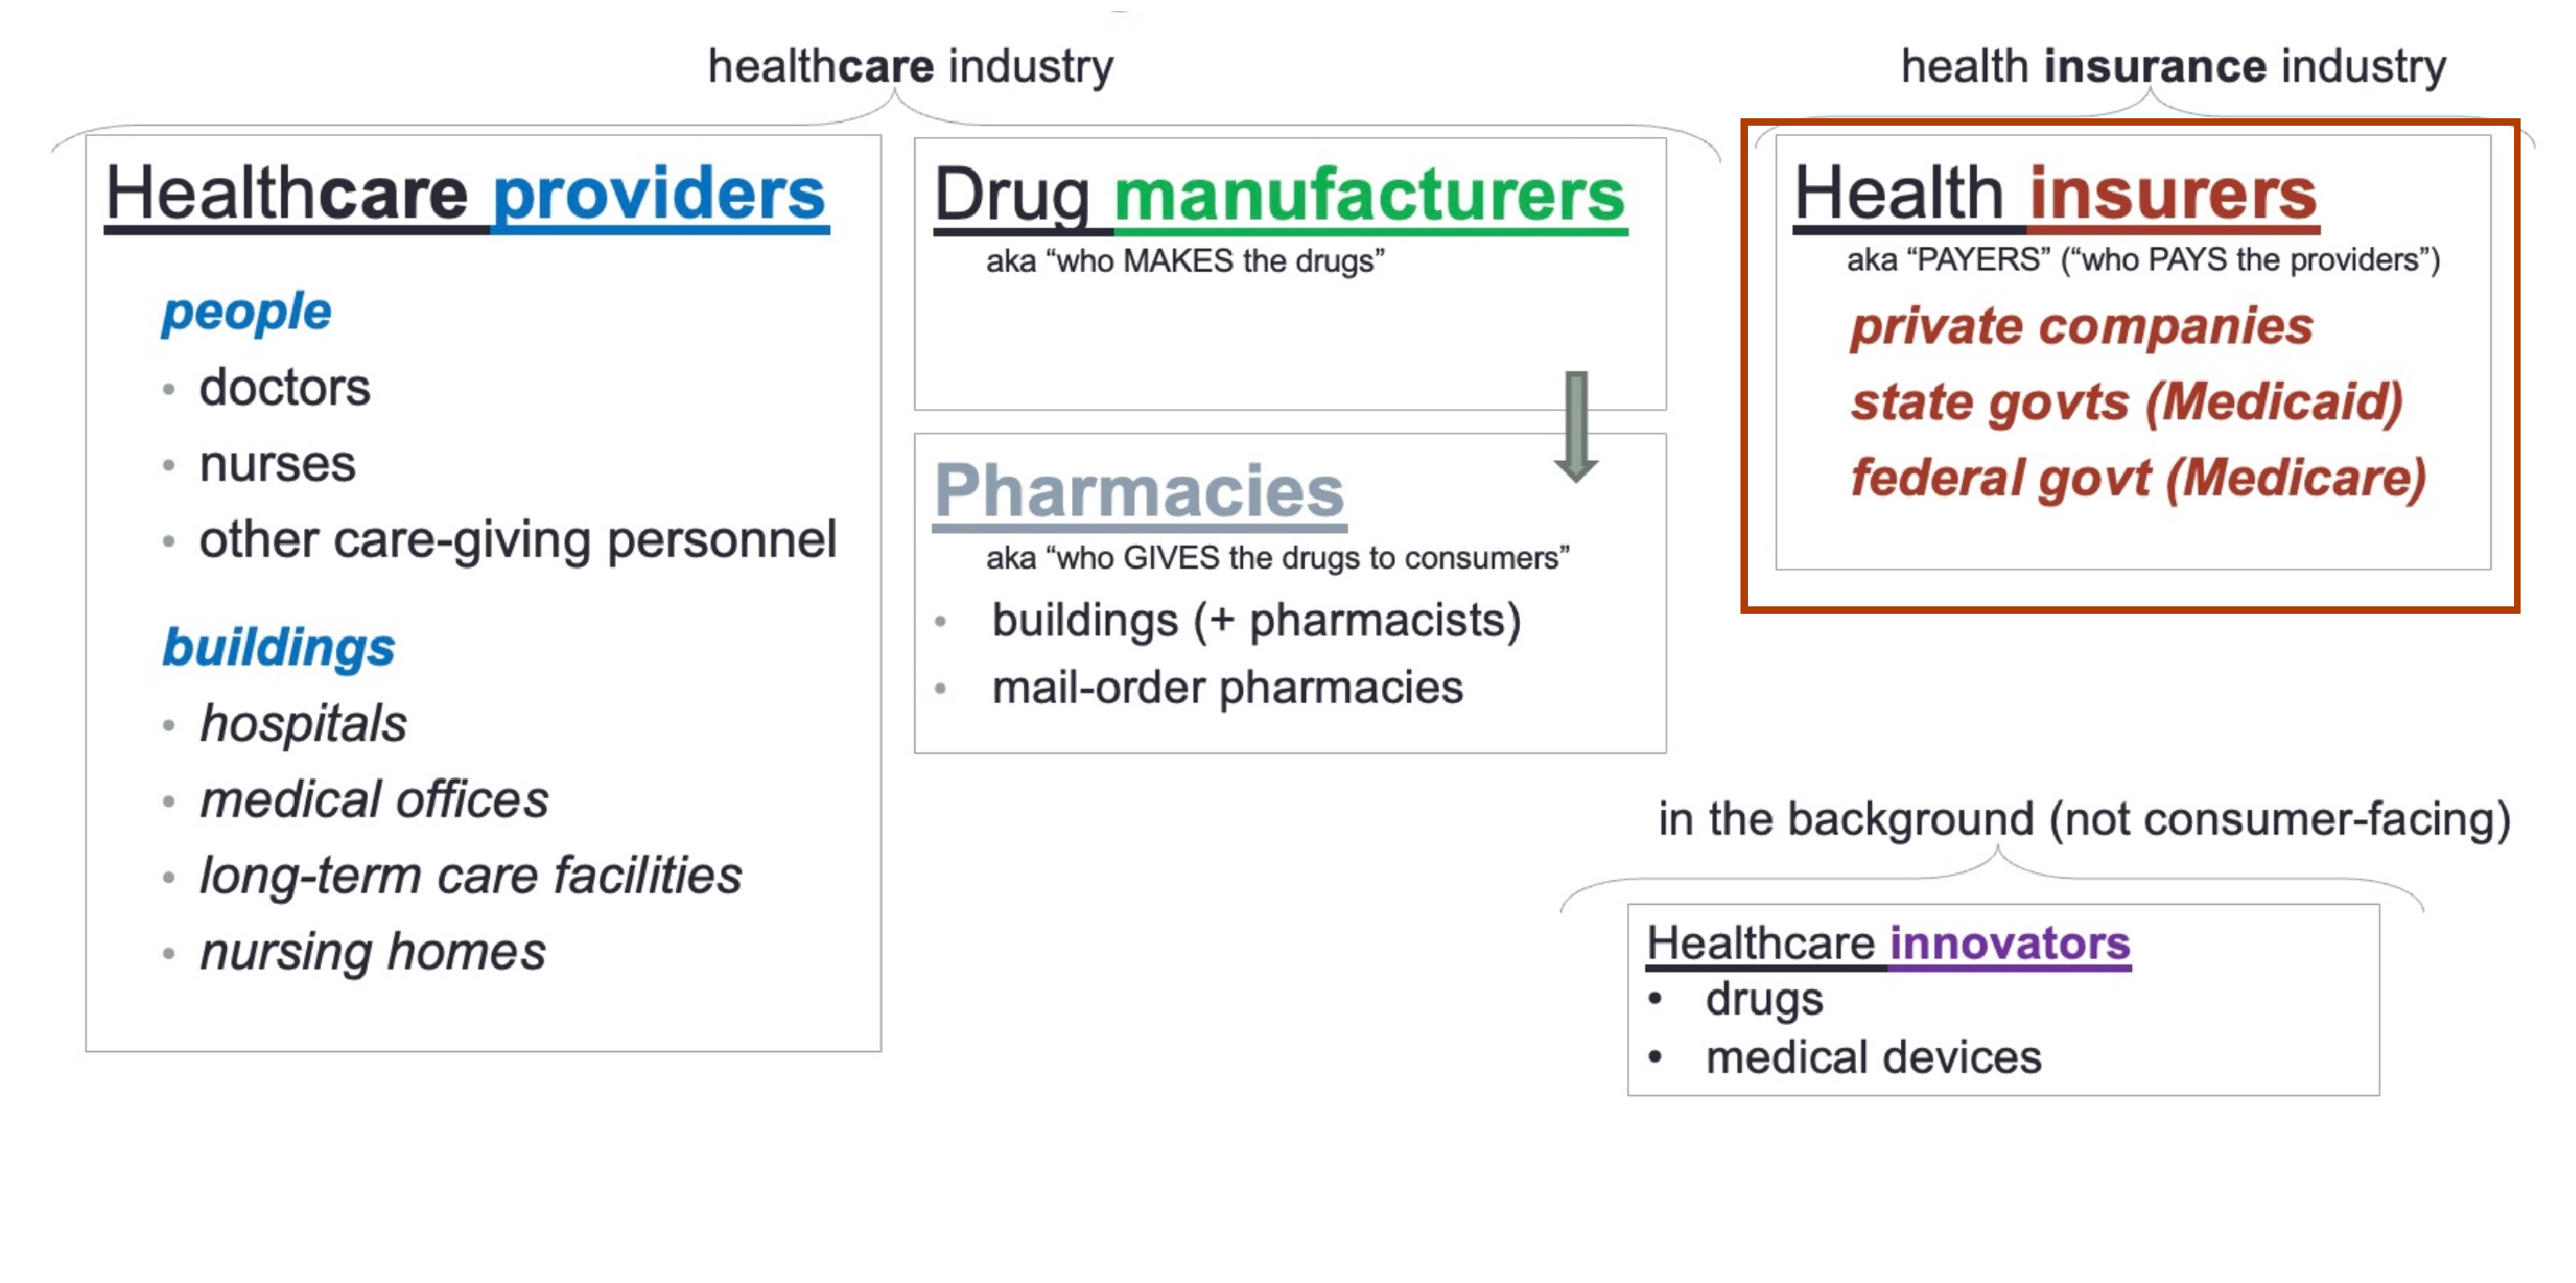
\includegraphics[height=0.9\textheight]{input/marone_UShealthcaresystem.pdf}
    \end{center}
\end{frame}
%---------------------------------------------------------------------

%---------------------------------------------------------------------
\begin{frame}{The U.S. healthcare system}
    \vspace{-7mm}
    \begin{center}
        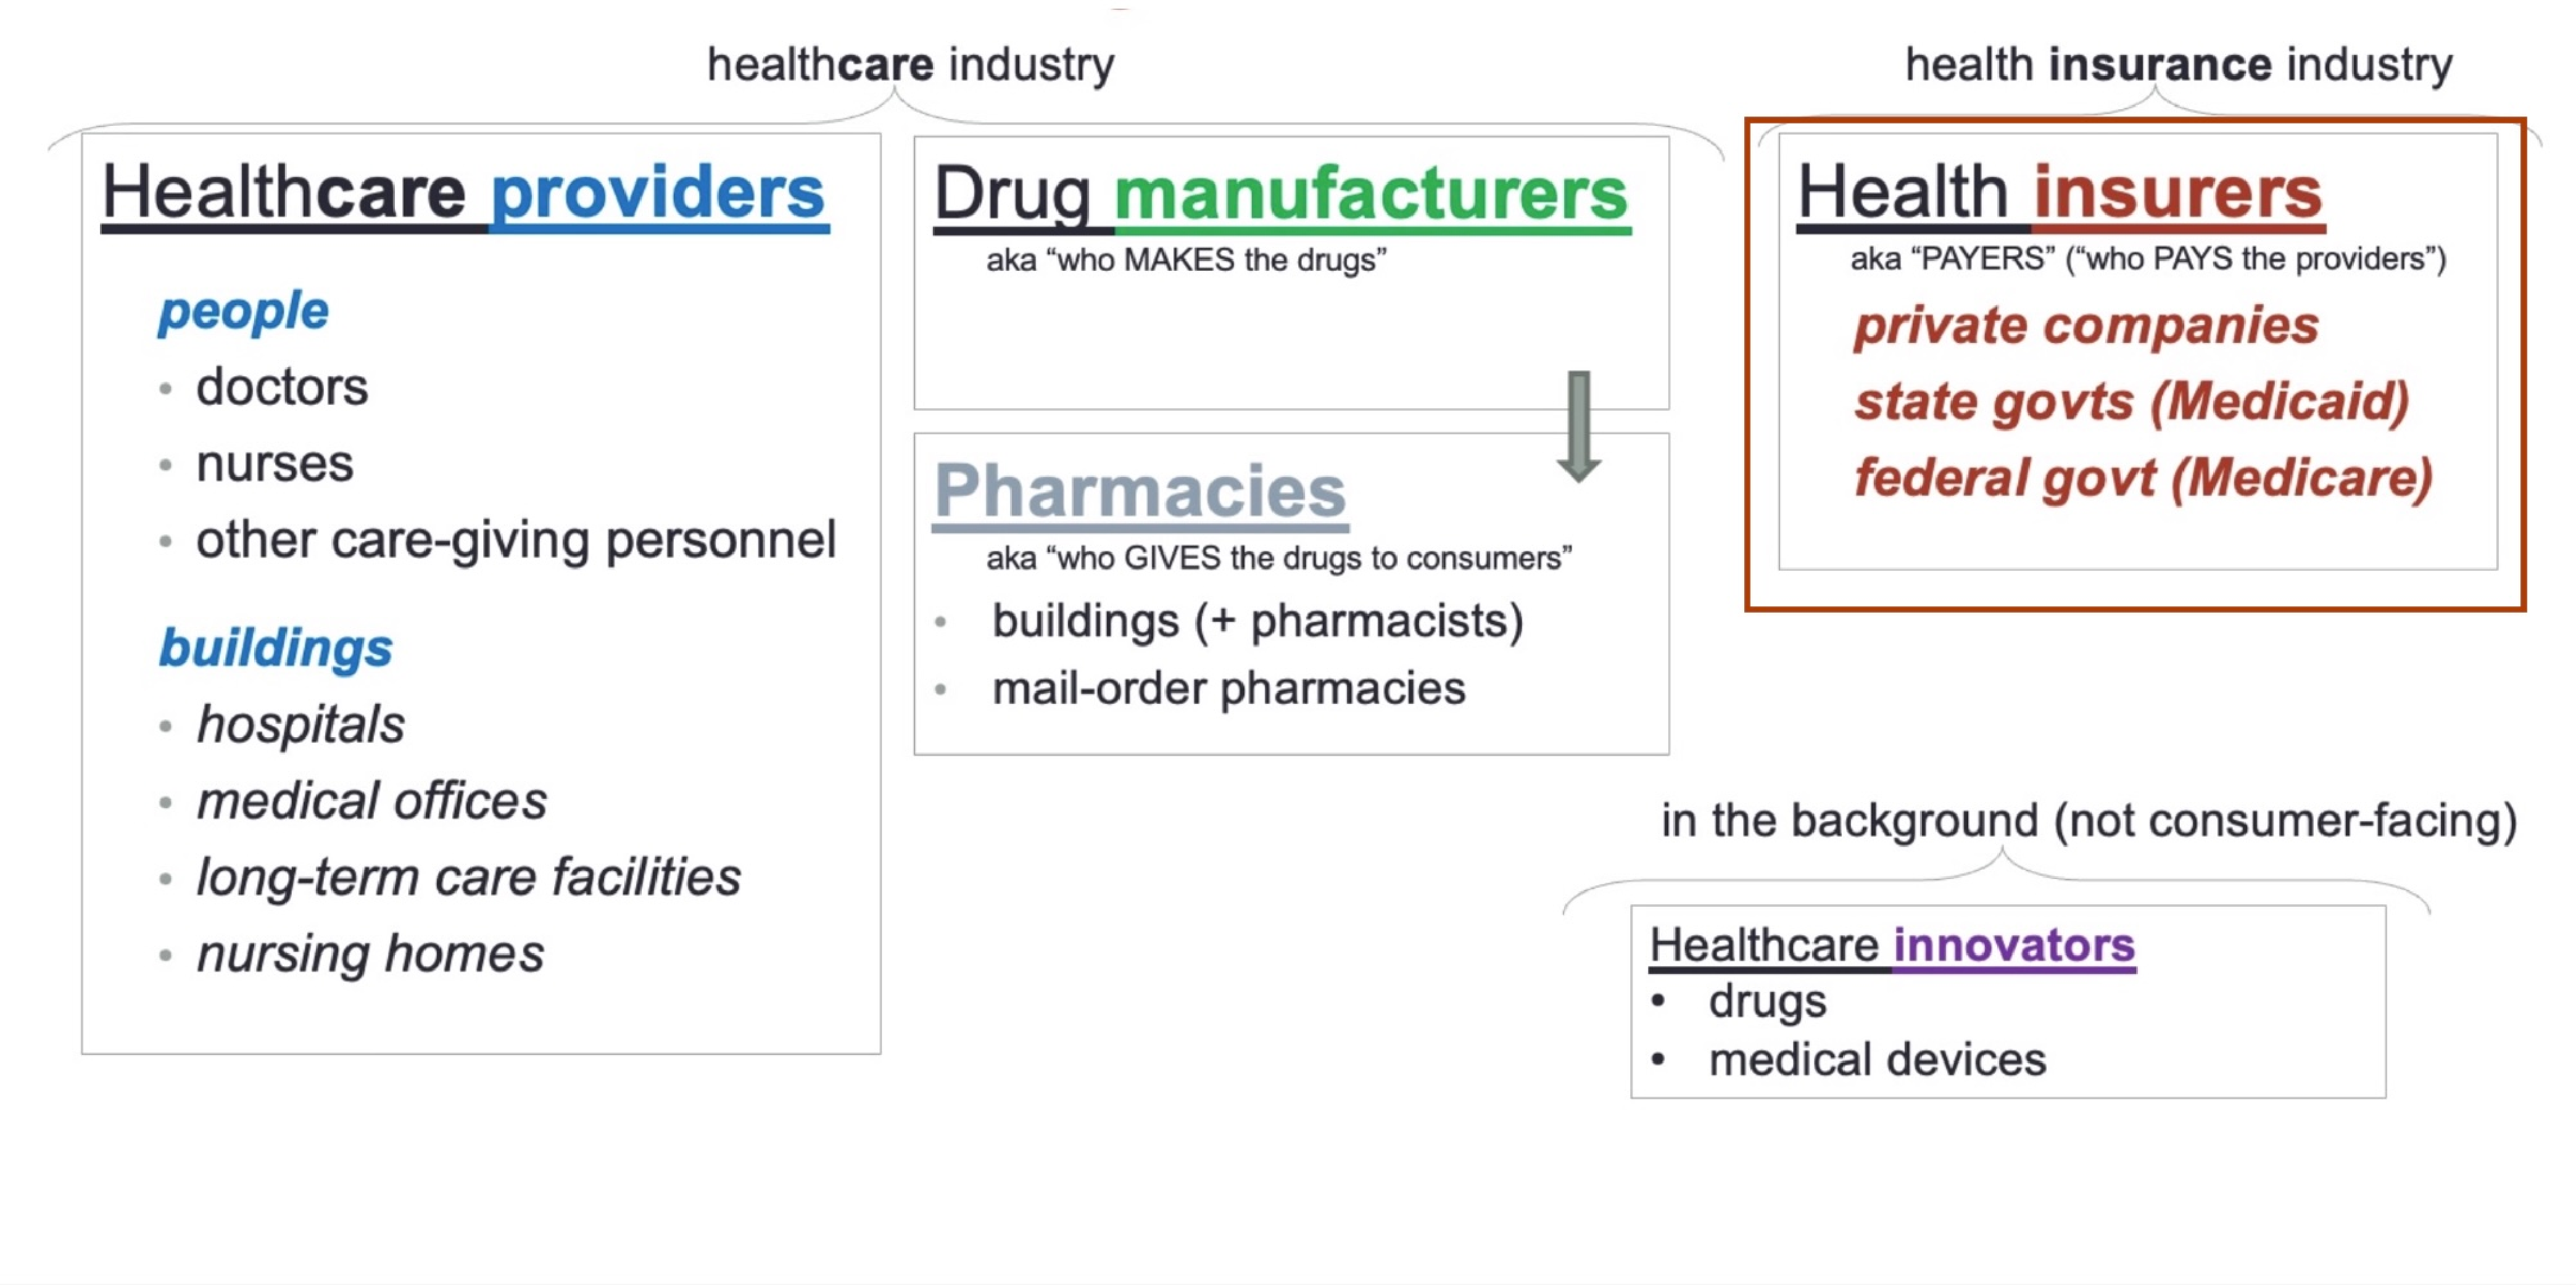
\includegraphics[height=0.9\textheight]{input/marone_UShealthcaresystem_focusinsurers.pdf}
    \end{center}
\end{frame}
%---------------------------------------------------------------------

%---------------------------------------------------------------------
\begin{frame}{}
    \vspace{-5mm}
    \begin{center}
        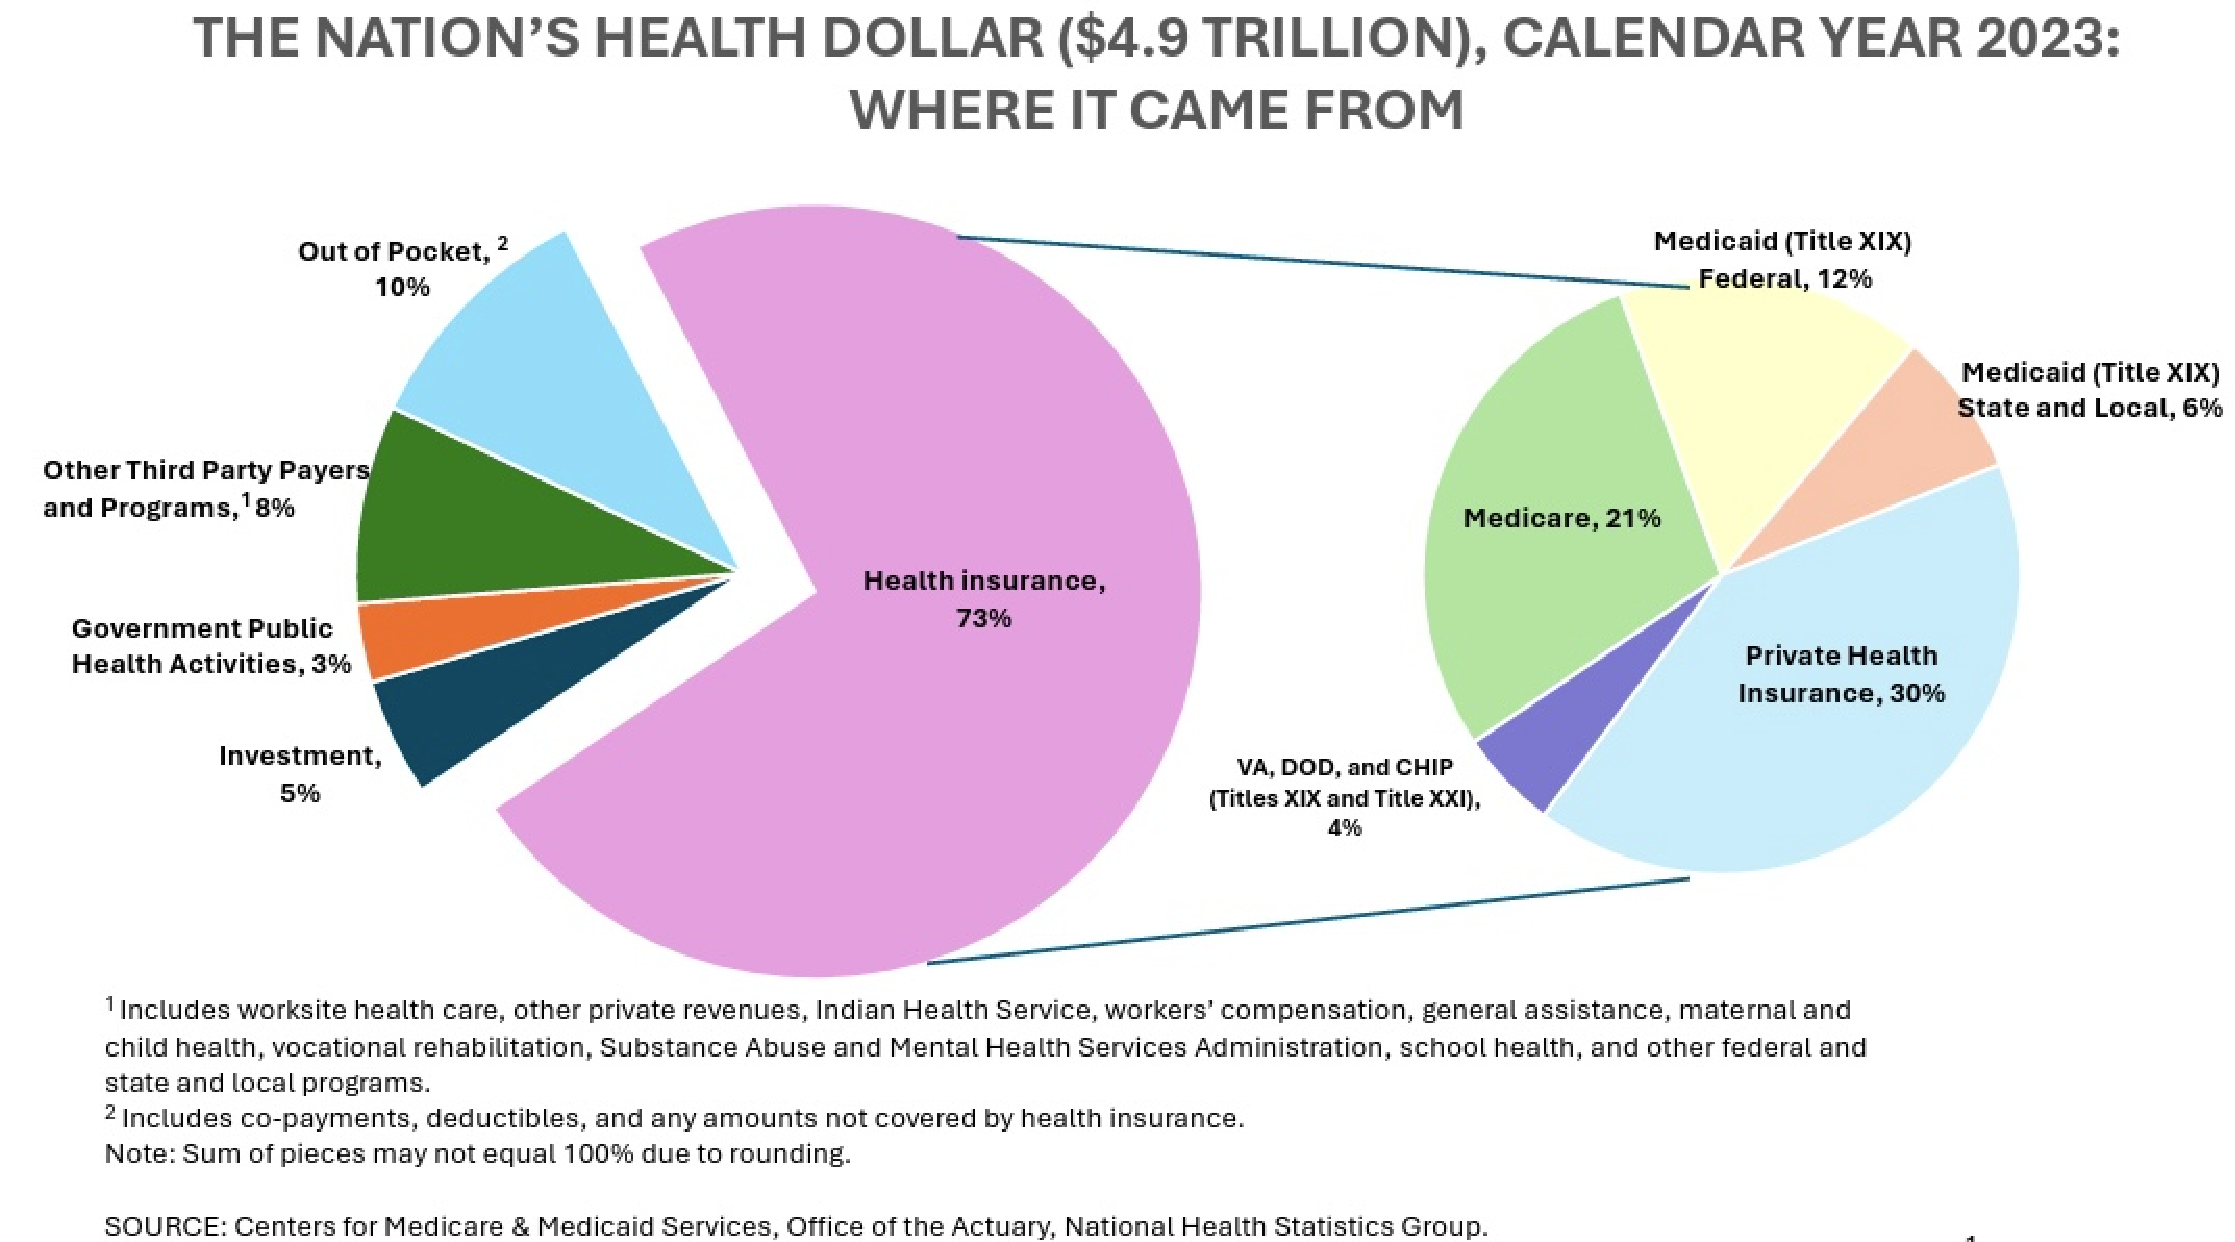
\includegraphics[height=0.95\textheight]{input/CMS_where_it_went2023_s1.pdf}
    \end{center}
    \vspace{-5mm}

    {\tiny Source: \href{https://www.cms.gov/files/document/nations-health-dollar-where-it-came-where-it-went.pdf}{CMS}.}
\end{frame}
%---------------------------------------------------------------------

%---------------------------------------------------------------------
\begin{frame}{Sources of health insurance coverage}
    \vspace{-1mm}
    \begin{center}
        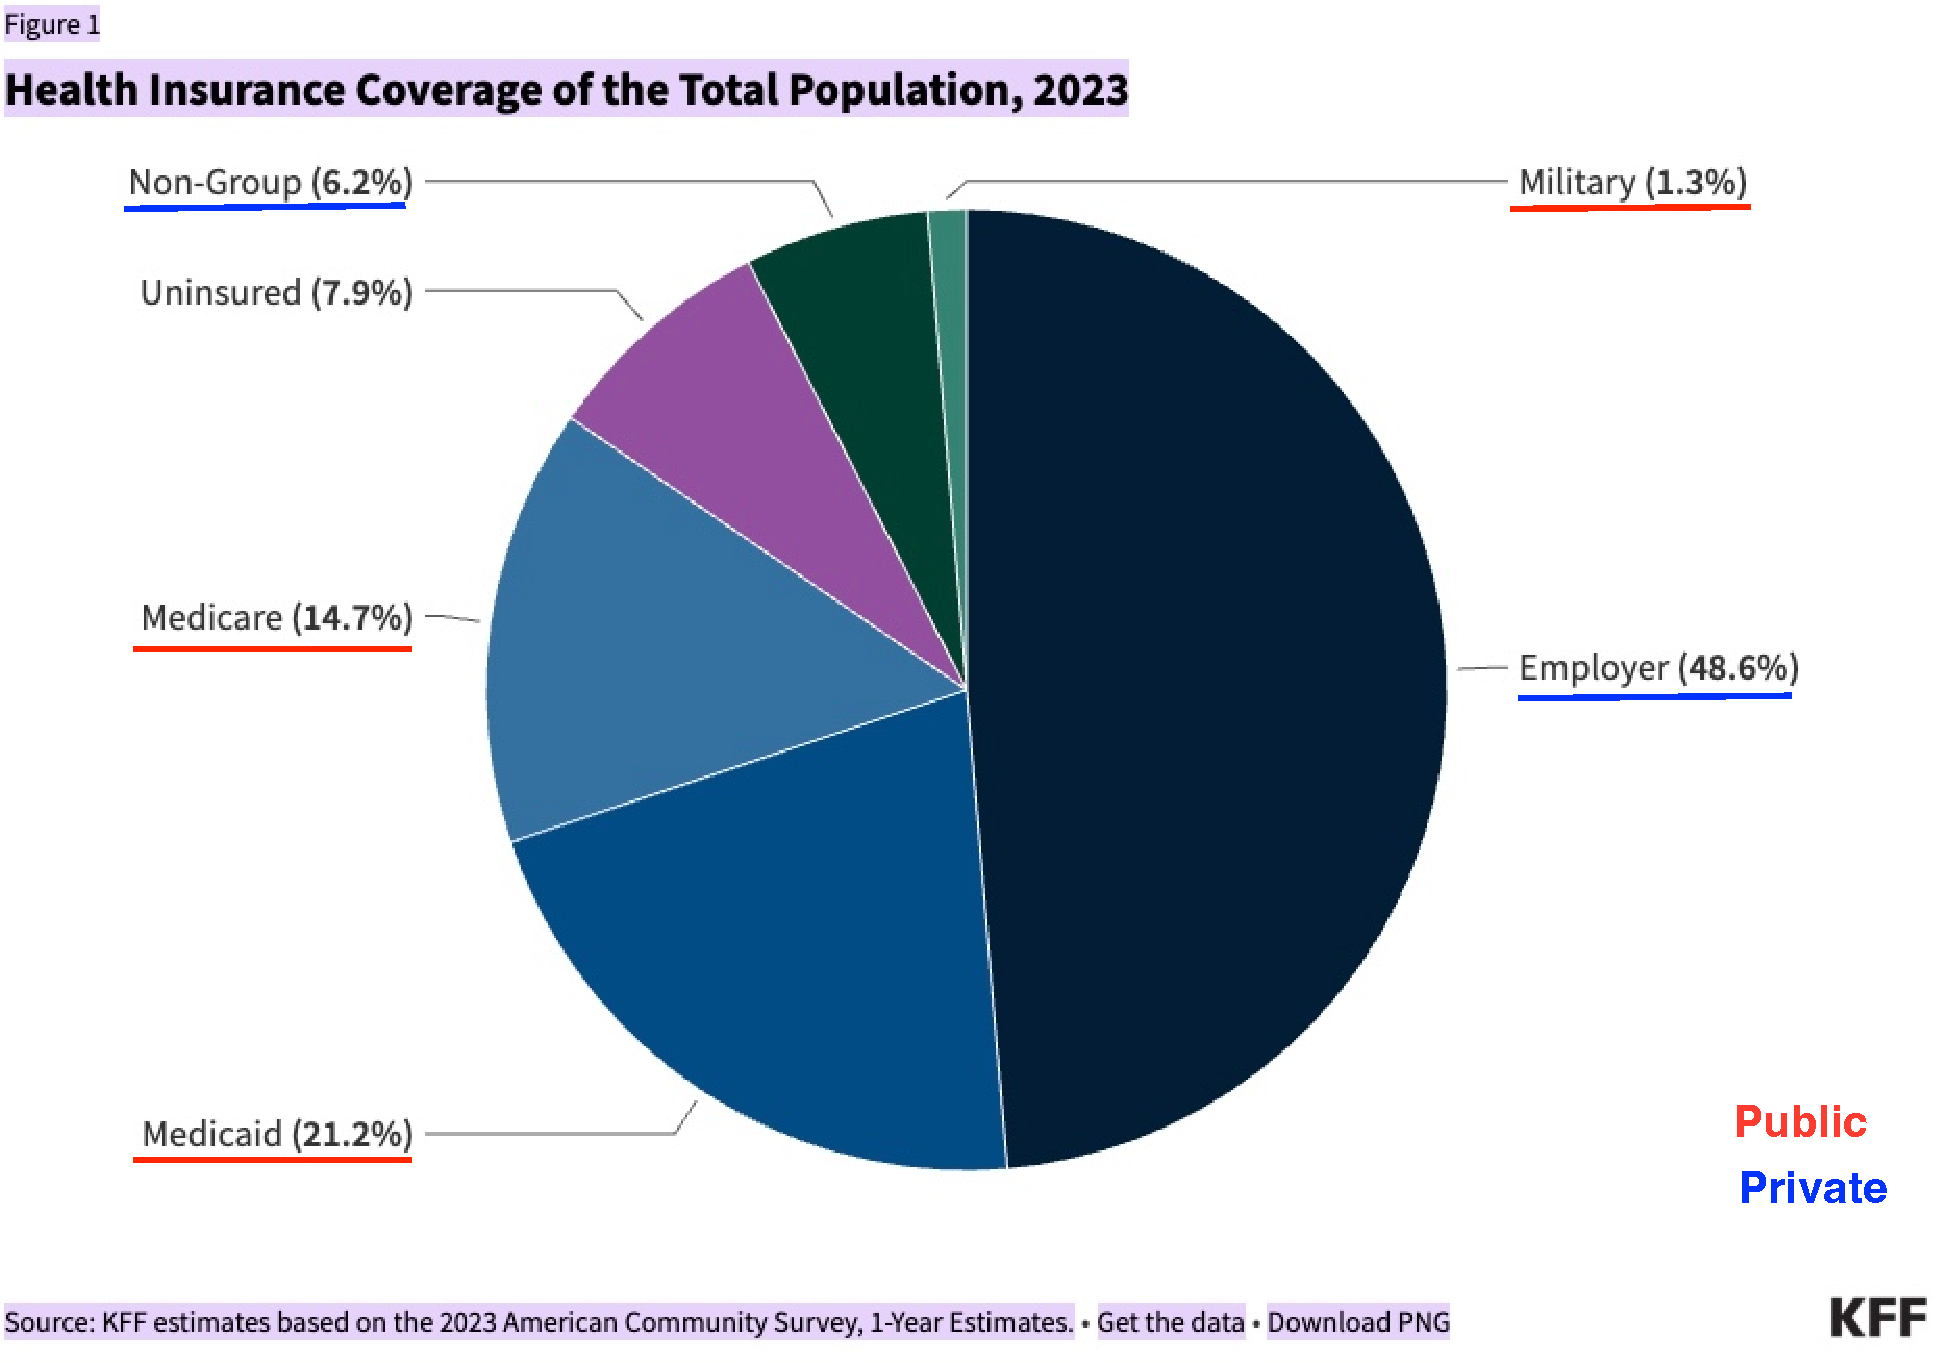
\includegraphics[height=0.85\textheight]{input/KFF_healthinsurancecoverage2023.pdf}
    \end{center}
\vspace{-5mm}

{\tiny Source: \href{https://www.kff.org/uninsured/health-policy-101-the-uninsured-population-and-health-coverage/?entry=table-of-contents-who-is-uninsured-in-the-united-states}{KFF website}.}
\end{frame}
%---------------------------------------------------------------------

%---------------------------------------------------------------------
\begin{frame}{Sources of health insurance coverage}
    \vspace{-1mm}
    \begin{center}
        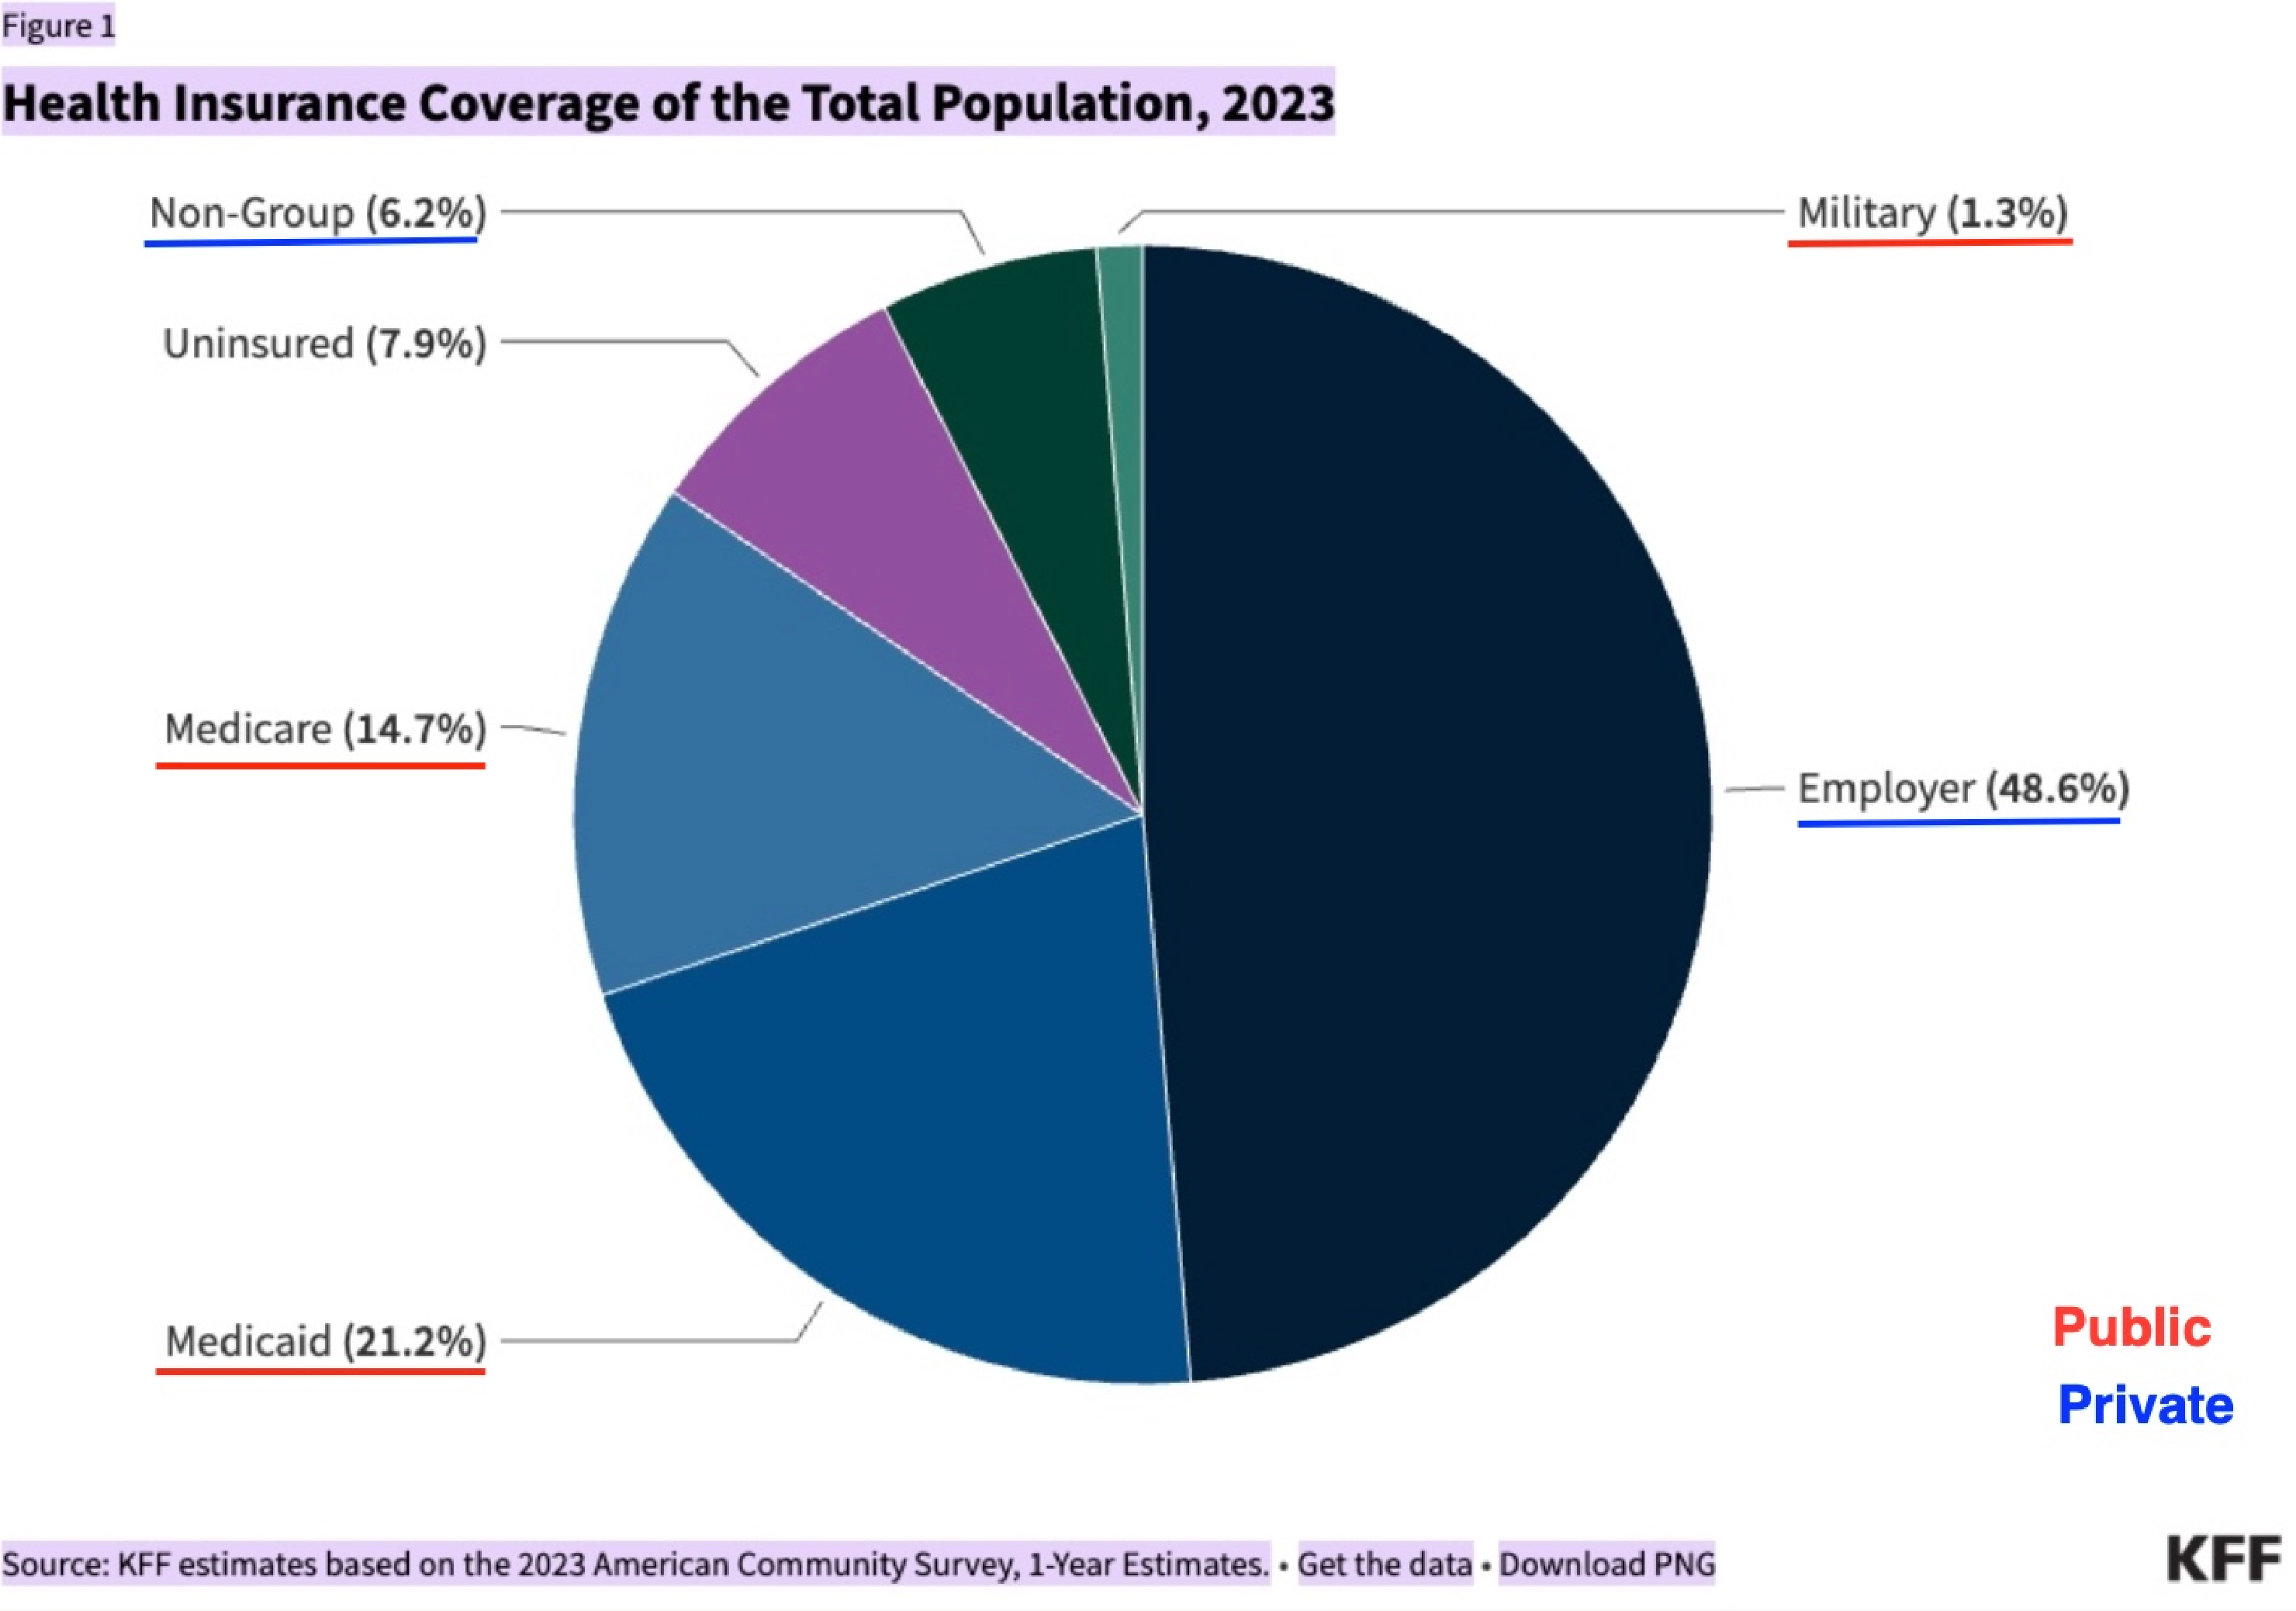
\includegraphics[height=0.85\textheight]{input/KFF_healthinsurancecoverage2023_highlights.pdf}
    \end{center}
\vspace{-5mm}

{\tiny Source: \href{https://www.kff.org/uninsured/health-policy-101-the-uninsured-population-and-health-coverage/?entry=table-of-contents-who-is-uninsured-in-the-united-states}{KFF website}.}
\end{frame}
%---------------------------------------------------------------------

%---------------------------------------------------------------------
\begin{frame}{}
    \begin{center}
    \Large \textcolor{maroon}{A bit of history}
    \end{center}

\end{frame}
%---------------------------------------------------------------------
%---------------------------------------------------------------------
\begin{frame}{A bit of healthcare history...}
    \vspace{-5mm}
    \begin{center}
        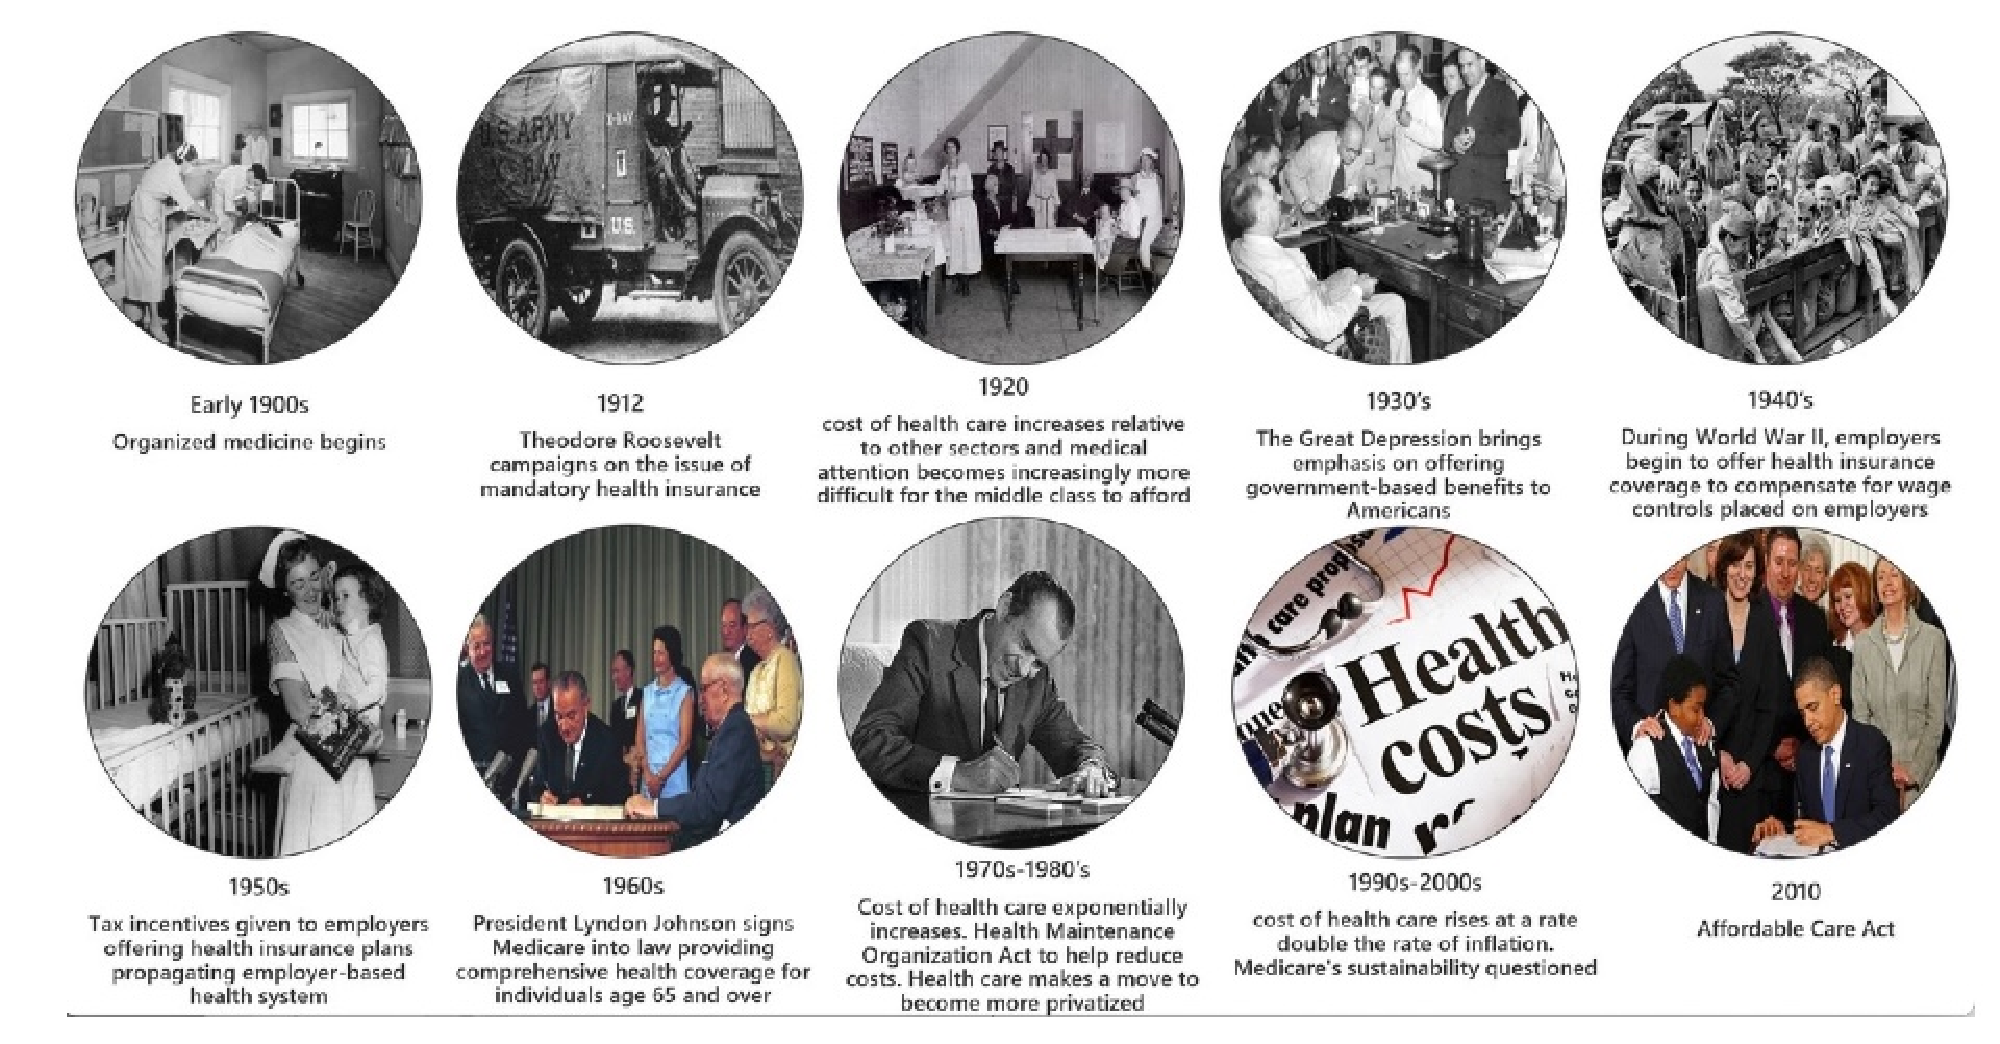
\includegraphics[height=0.9\textheight]{input/history_insurance.pdf}
    \end{center}
\end{frame}
%---------------------------------------------------------------------

% ``organized medicine'' and the AMA

% AMA created in 1847 in Philadelphia. Becomes a dominant force by early 1900s.

% Before: anyone could claim to be a doctor, low quality med schools,  competition was fierce, and competitition with alternative practices of medicine

% Organized medicine:
% - formed professional Association
% - established licensing standards
% ==> State medical boards + scope of practice
% - controlled medical education
% Flexner report (1910) closed many schools, standardized medical education, required hospital based instruction
% ==> Created entry barriers into medicine → fewer physicians → higher professional status and incomes.

% Overall:
% - control of entry into profession
% - pricing: bargaining power with hospitals
% - fought against national health insurance proposals
% why? threat to autonomy, income, amd control over medical practice


% 1930s (New Deal) Roosevelt entertains health insurance in social security, AMA pressure keeps it out

% 1965: physicians ended up accepting because fee-for-service, they seat on board to determine these fees, and no government employment of docs

%---------------------------------------------------------------------
\begin{frame}{A bit of healthcare history...}
    \vspace{-5mm}
    \begin{center}
        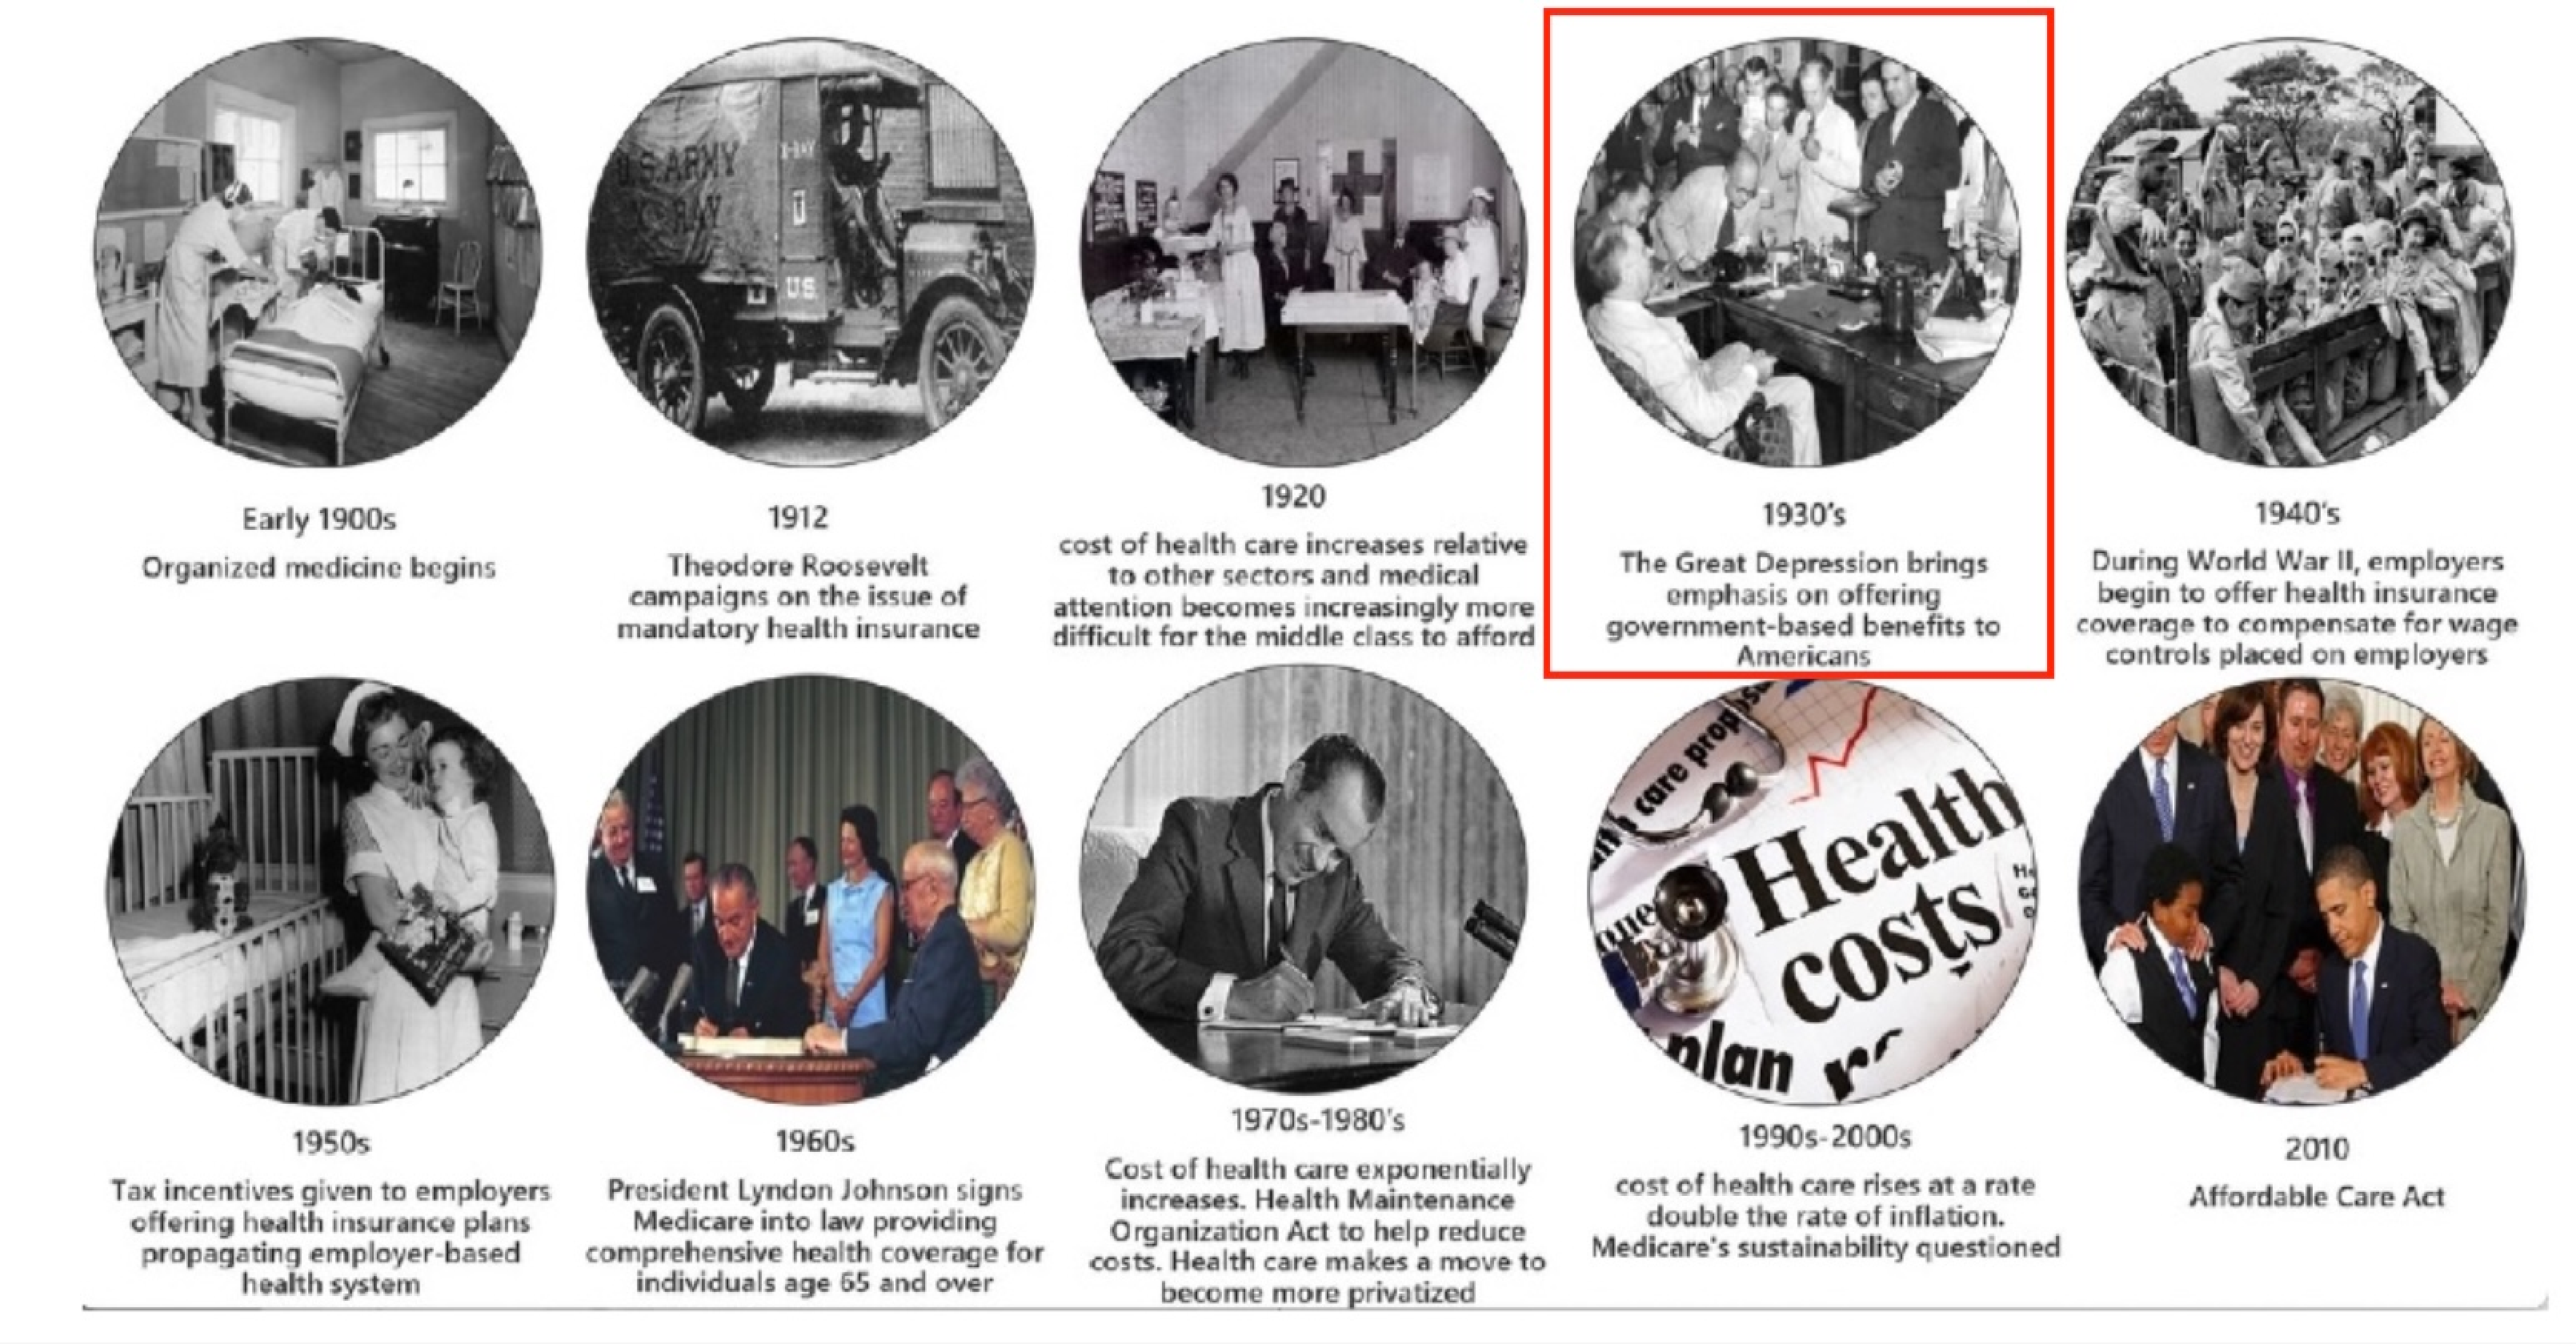
\includegraphics[height=0.9\textheight]{input/history_insurance_highlight.pdf}
    \end{center}
\end{frame}
%---------------------------------------------------------------------

%---------------------------------------------------------------------
\begin{frame}{Hospitalization insurance: Blue Cross}

    \begin{itemize}
        \item \textcolor{navy}{Blue Cross}
        \begin{itemize}
            \item Dallas 1929: prepaid hospital coverage for Dallas school teachers
            \item Started at Baylor hospital, spread across others, and offered joint hospitalization insurance
            \item Sold through employers
            %for hospitals: great depression decreased bed utilization + preventing hospital competition
            \item Strong support from AHA: Blue Cross symbol in 1939
            \item 25 states voted that these plans be tax-exempt charitable organizations
        \end{itemize}
        % not the first effort but the effort that caught "fire"
        \vspace{3mm}

        \item Private plans
        \begin{itemize}
            \item Learned from the Blue Cross experience
            \item Surpassed them in heads covered in 1951
        \end{itemize}
    \end{itemize}
\end{frame}

%---------------------------------------------------------------------
\begin{frame}{Physician services coverage: Blue Shield}

    \begin{columns}[T]   % T = top alignment
        % ---------------- LEFT COLUMN ----------------
        \begin{column}{0.7\textwidth}
            \begin{itemize}
                \item \textcolor{navy}{Blue Shield}
                \begin{itemize}
                    \item California and Michigan 1939
                    \item Coverage for office visits, house calls, and in-hospital physician services
                    \item Controlled by physicians
                    \item Blue Cross assistance to combat private insurers who were bundling
                \end{itemize}
                %AMA initially very opposed by (1) low demand from depression
                %(2) calls for government insurance they didnt like so needed to propose an alternative
                %(3) scared that Blue Cross would cover in-hospital physician services so they would be cut out
            \end{itemize}
            \vspace{3mm}
        
            $\implies$ By 1940, 20 million Americans had some form of health insurance\\
            $\implies$ 1982: the \textcolor{navy}{Blue Cross Blue Shield} Association is formed
        \end{column}
    
        % ---------------- RIGHT COLUMN ----------------
        \begin{column}{0.3\textwidth}
            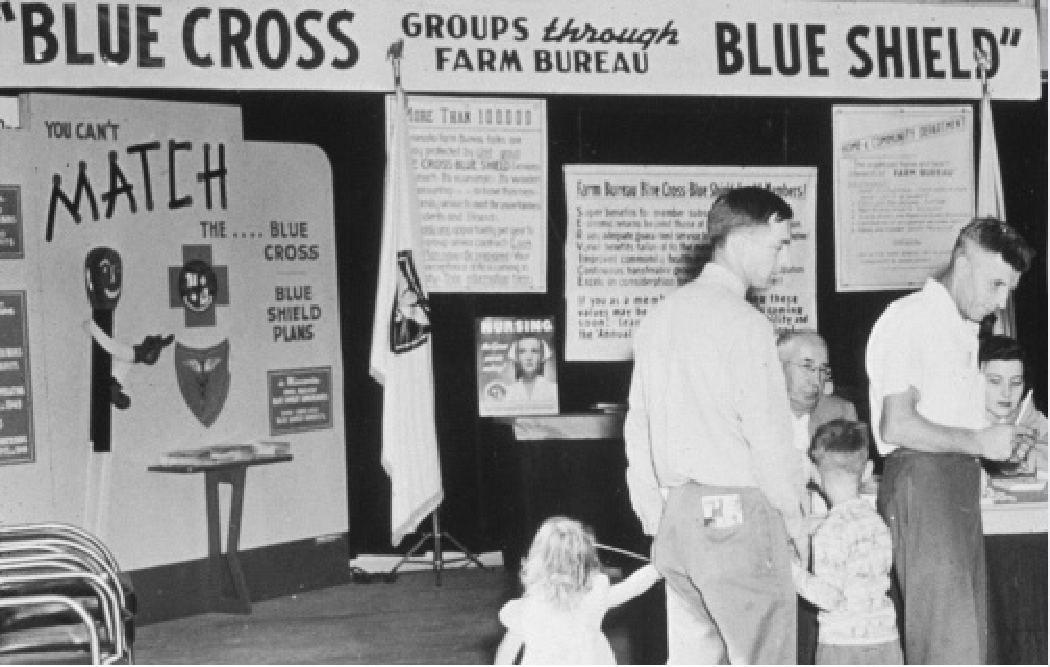
\includegraphics[width=1.1\textwidth]{input/BCBS_historical_image.pdf}\\
            \vspace{25mm}
            
\includegraphics[width=0.9\textwidth]{input/BCBS_logo.pdf}

        \end{column}
    \end{columns}
\end{frame}
%---------------------------------------------------------------------
\begin{frame}{Why then?}

    \only<1>{
        \begin{itemize}
            \item Great depression
            \begin{itemize}
                \item Decreased bed utilization and low demand for physician services
            \end{itemize}
            \vspace{3mm}
        \end{itemize}

        \vspace{56mm}
    }
    \only<2>{
        \begin{itemize}
            \item Great depression
            \begin{itemize}
                \item Decreased bed utilization and low demand for physician services
            \end{itemize}
            \vspace{3mm}
    
            \item Push for government insurance
            \begin{itemize}
                \item Fear of losing independence for doctors (AMA)\\
                $\implies$ Need to propose an alternative
            \end{itemize}
            \vspace{3mm}
        \end{itemize}
        \vspace{34mm}

    }

    \only<3>{
        \begin{itemize}
            \item Great depression
            \begin{itemize}
                \item Decreased bed utilization and low demand for physician services
            \end{itemize}
            \vspace{3mm}
    
            \item Push for government insurance
            \begin{itemize}
                \item Fear of losing independence for doctors (AMA)\\
                $\implies$ Need to propose an alternative
            \end{itemize}
            \vspace{3mm}
    
            \item Response to competition
            \begin{itemize}
                \item From other hospitals (Blue Cross)
                \item From other insurance plans
                \begin{itemize}
                    \item Private insurers were bundling hospital and physician services coverage
                    \item Blue Shield: fear that Blue Cross would cover in-hospital physician services
                \end{itemize}
                $\implies$ Would have effectively cut out physicians
            \end{itemize}
        \end{itemize}
    }
    
\end{frame}

%---------------------------------------------------------------------

%---------------------------------------------------------------------
\begin{frame}{If you want to go further...}

    \begin{columns}[T]   % T = top alignment
        % ---------------- LEFT COLUMN ----------------
        \begin{column}{0.8\textwidth}
            \begin{itemize}
                \item[*] 
                \textit{The Social Transformation of American Medicine} by Paul Starr
    
                \vspace{18mm}
    
                \item[*] 
                \textit{Reinventing American Health Care} by Ezechiel J. Emanuel
            \end{itemize}
    
        \end{column}
    
        % ---------------- RIGHT COLUMN ----------------
        \begin{column}{0.2\textwidth}
            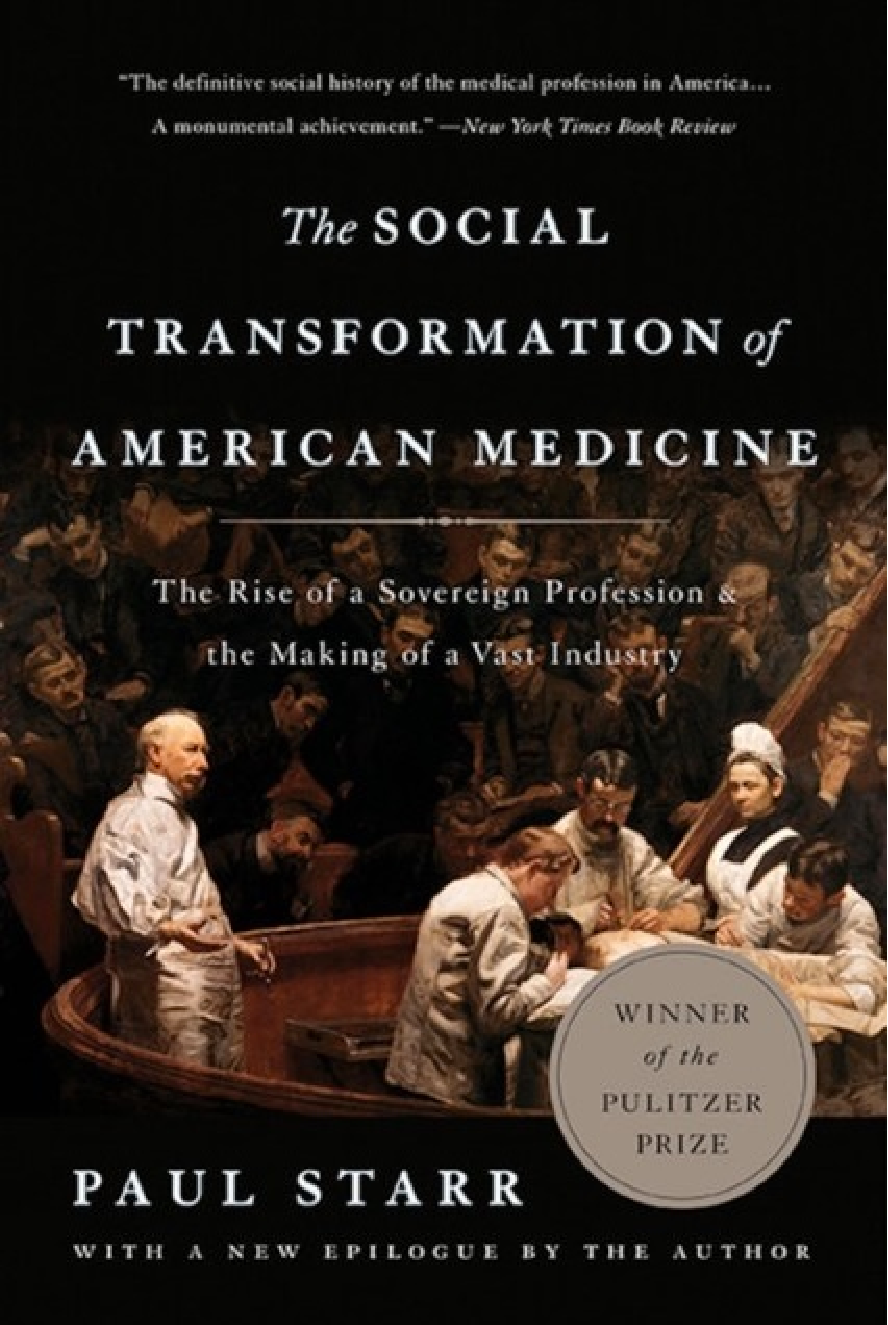
\includegraphics[width=0.7\textwidth]{input/book_starr.pdf}
    
            \vspace{4mm}
    
            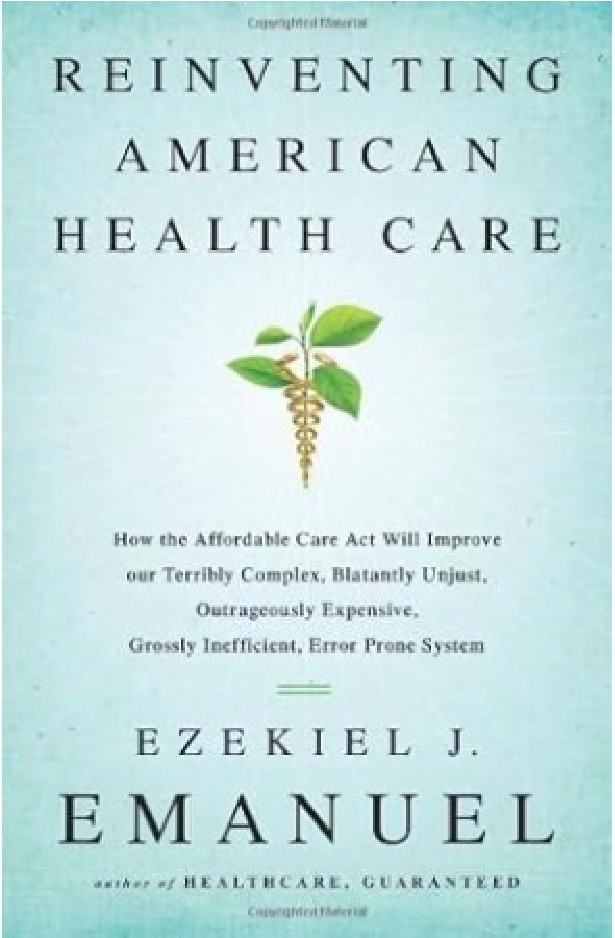
\includegraphics[width=0.7\textwidth]{input/book_emanuel.pdf}
        \end{column}
    \end{columns}

\end{frame}
%---------------------------------------------------------------------
\begin{frame}{The turning point for \newbold{employer-based insurance}}
    \begin{itemize}
        \item \newbold{World War II}: need to stabilize prices and wages. Labor shortage.
        \begin{itemize}
            \item 1942: \newbold{Stabilization Act}. Salaries and wages are frozen.
            \begin{itemize}
                \item Is health insurance included as wage or salaries?\\
                $\implies$ National War Labor Board says no... \\
                ... as long as does not exceed 5\% of the value of the wage
            \end{itemize}

            \item Doubling down:
            \begin{itemize}
                \item 1945: plans can't be canceled after the war
                \item 1949: unions should negotiate for fringe benefits, including health insurance
                \item IRS 1954: tax exclusion of health insurance in workers income
                %payroll tax + value of beenfit more than one dollar of income
                %"Cadillac" tax
            \end{itemize}
        \end{itemize}
    \end{itemize}
    \vspace{5mm}

    $\implies$ By 1950, two-thirds of working Americans has hospital stay coverage
    %$\implies$ Employer-sponsored health insurance firmly institutionalized

\end{frame}
%---------------------------------------------------------------------
\begin{frame}{Private health insurers}
    \begin{center}
        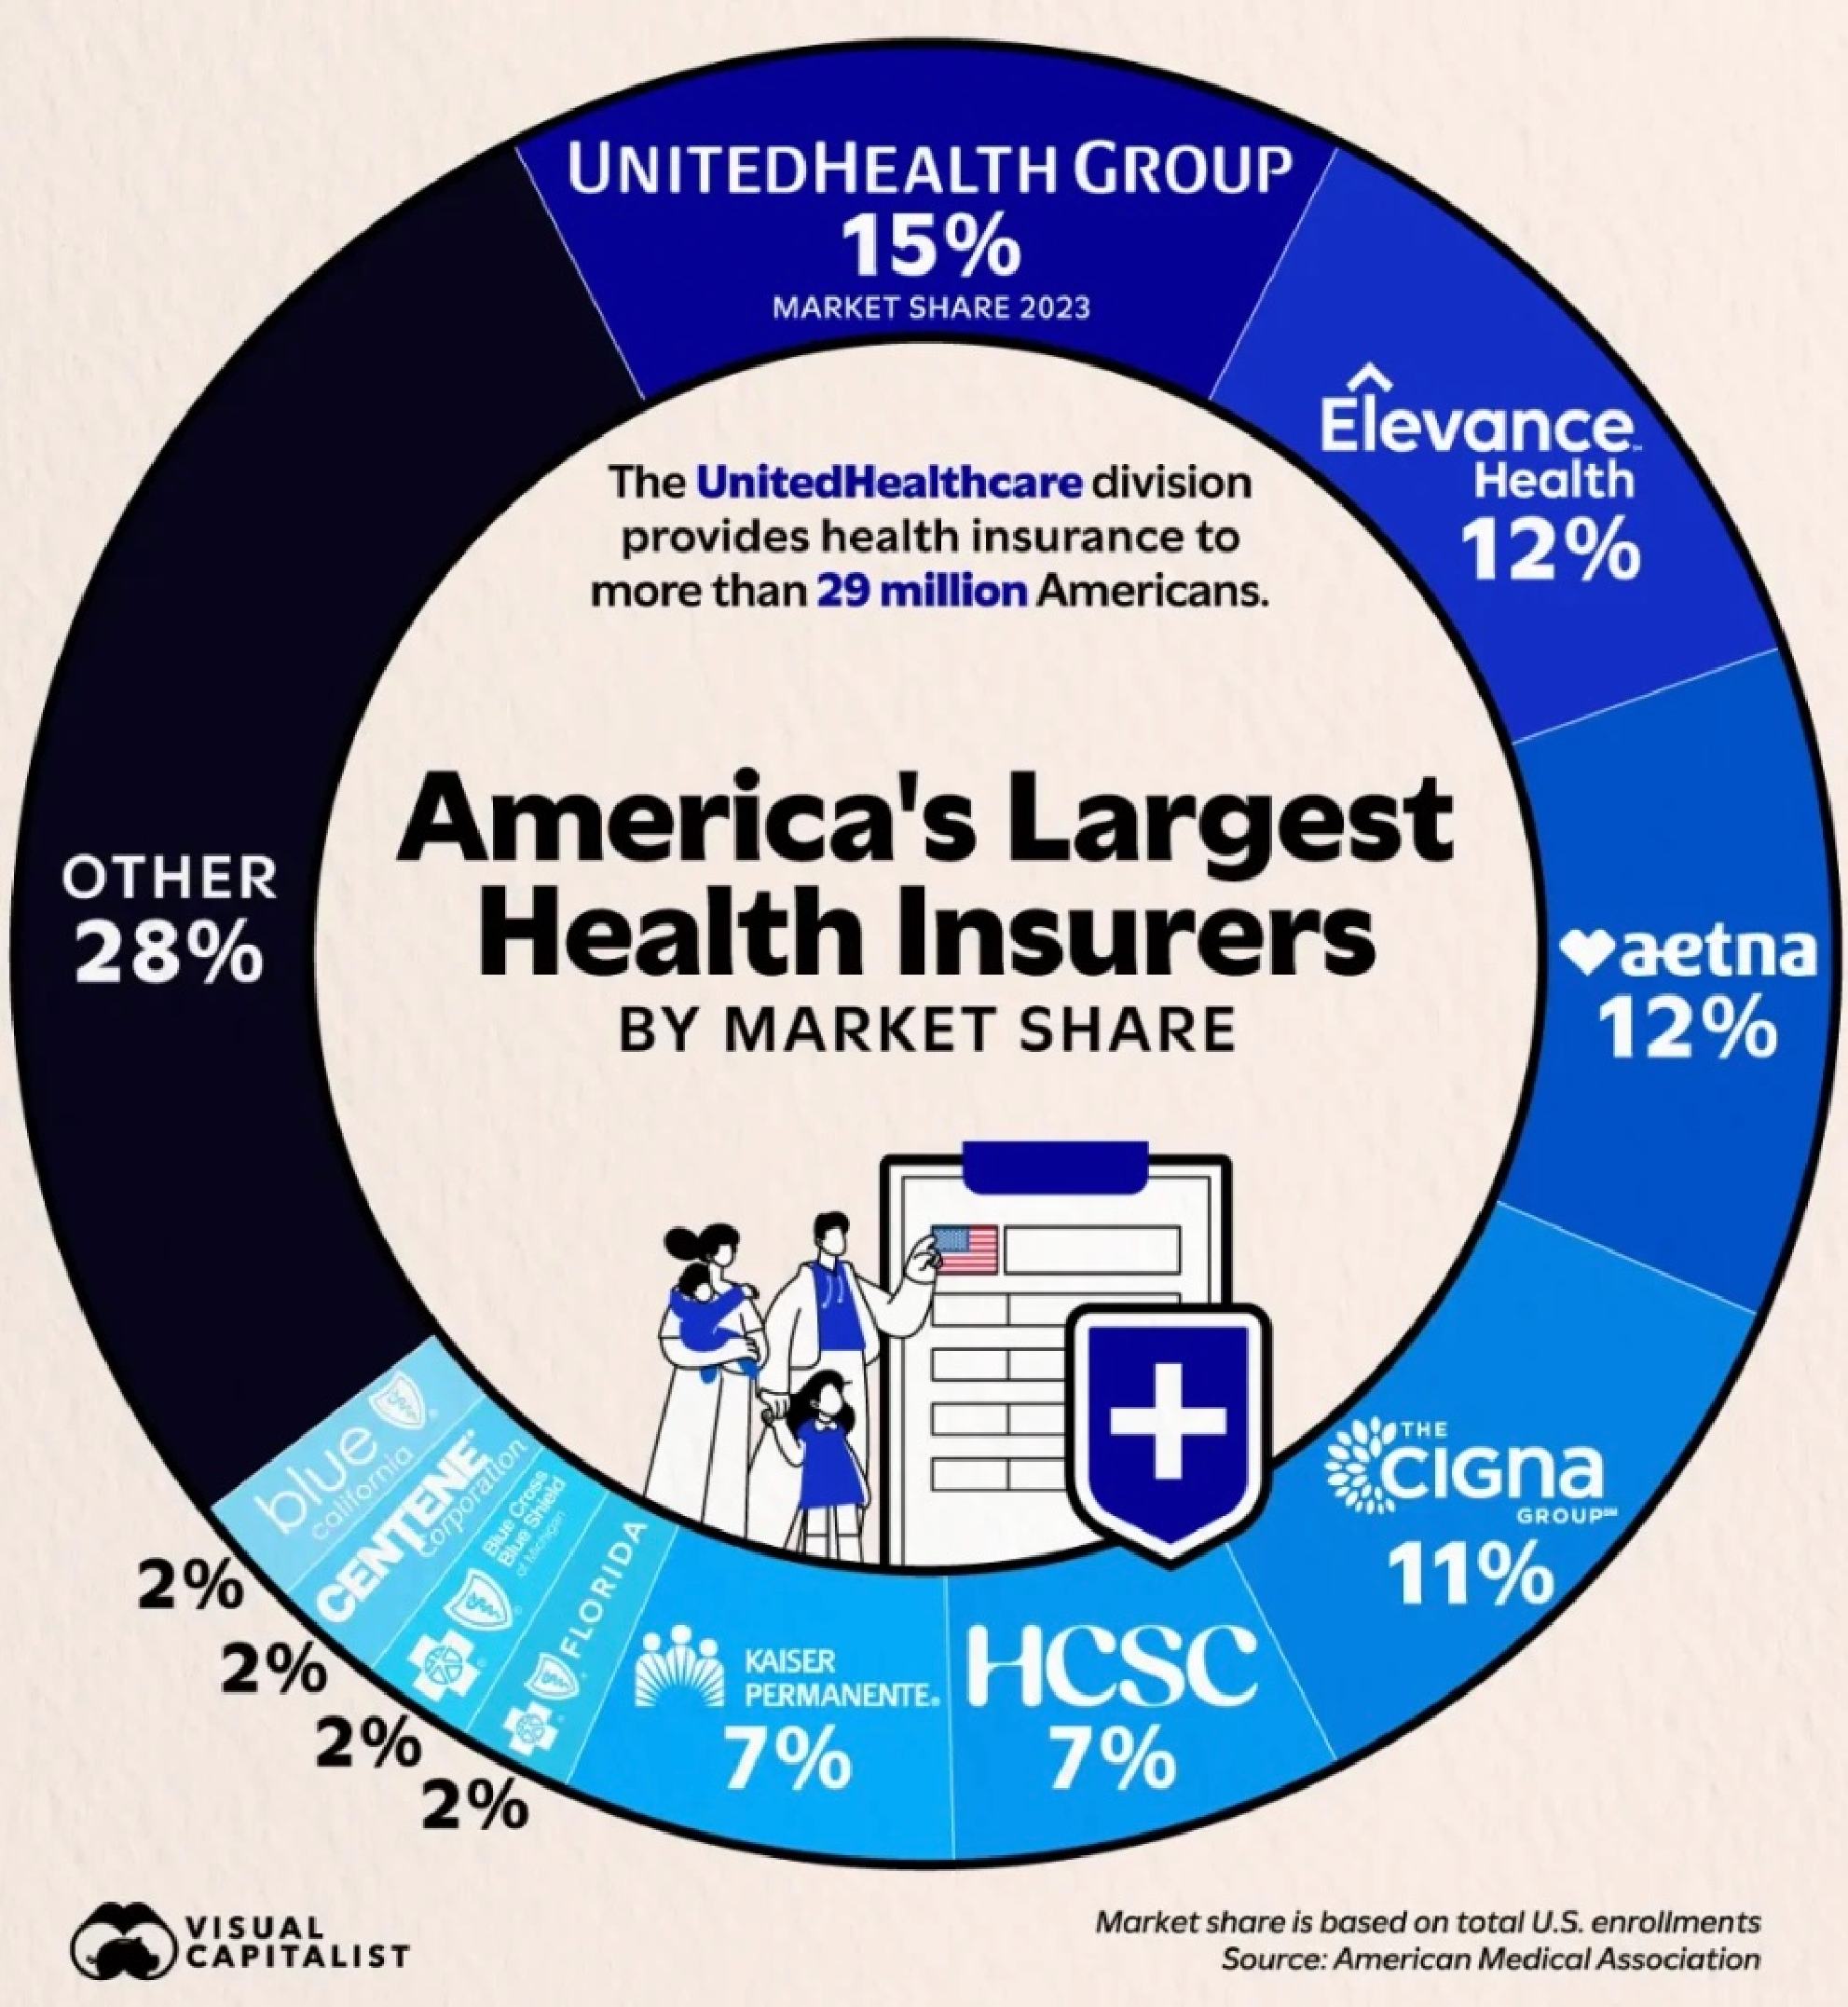
\includegraphics[height=0.9\textheight]{input/top_insurers2024.pdf}
    \end{center}
\end{frame}
%---------------------------------------------------------------------
\begin{frame}{}
    \begin{center}
        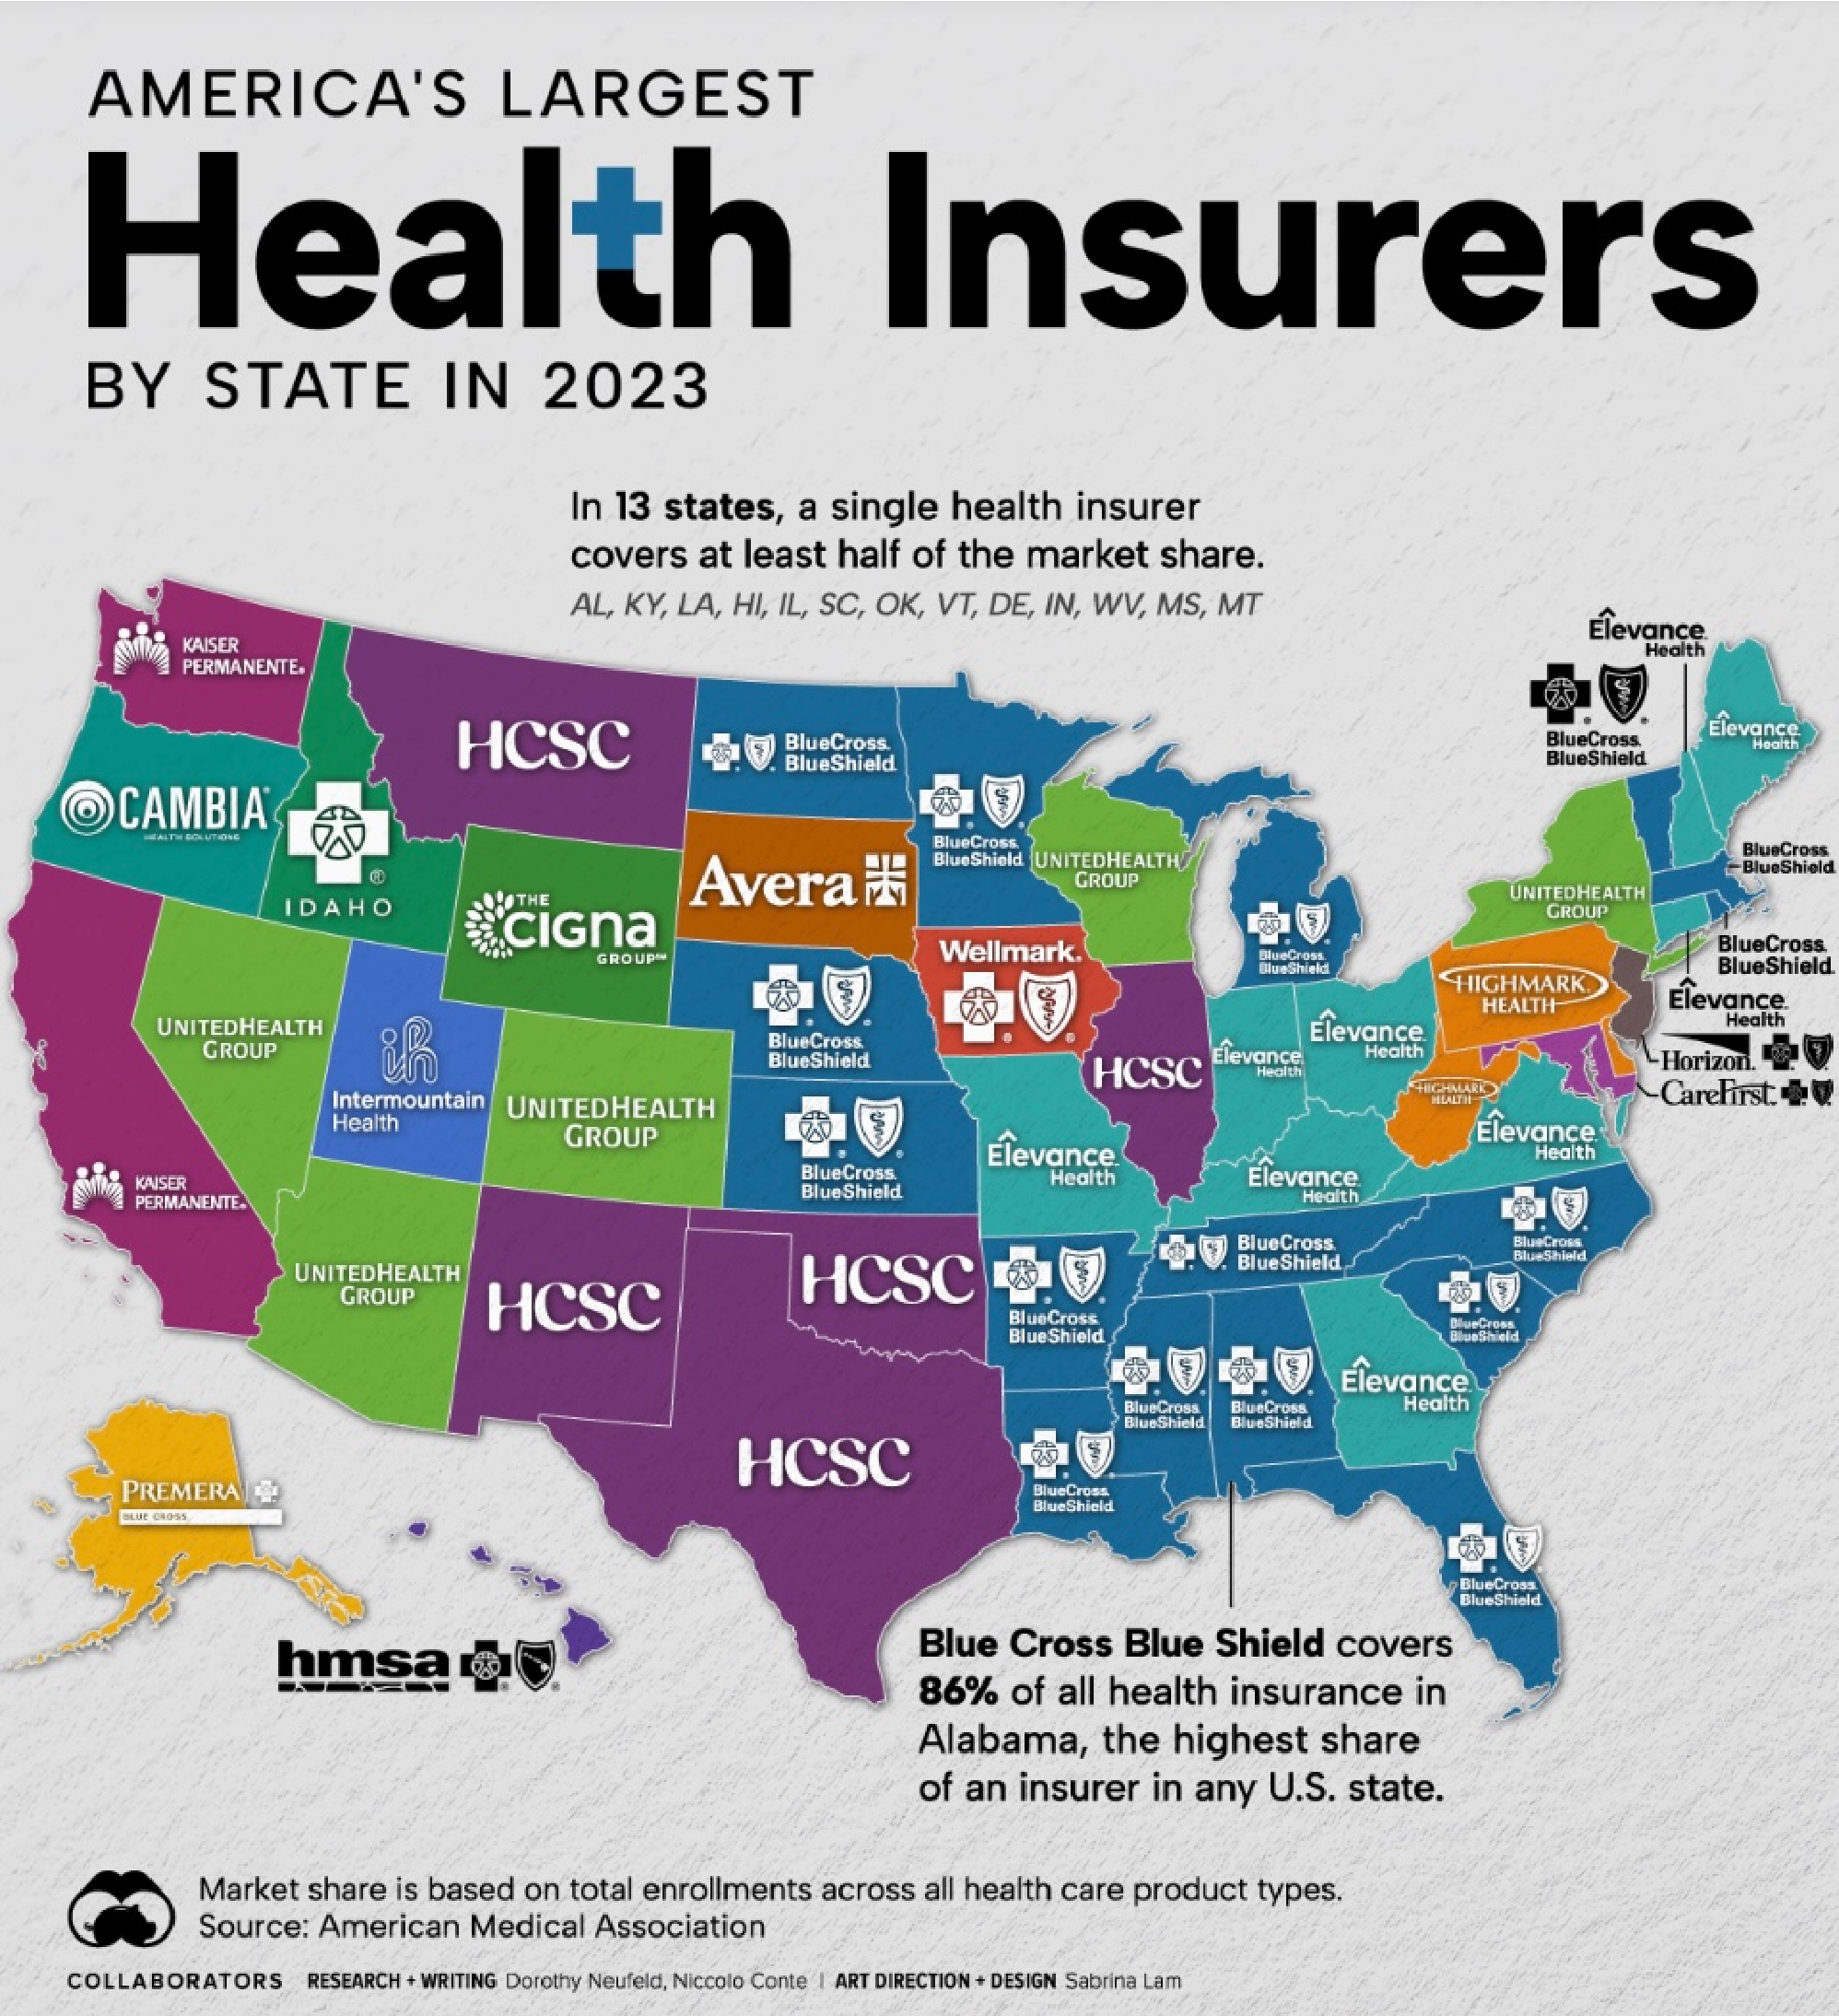
\includegraphics[height=0.9\textheight]{input/map_healthinsurers.pdf}
    \end{center}
    \vspace{-5mm}

    {\tiny Source: see \href{https://www.visualcapitalist.com/top-health-insurance-companies-by-state/}{here}.}
\end{frame}
%---------------------------------------------------------------------

%---------------------------------------------------------------------
\begin{frame}{A bit of healthcare history...}
    \vspace{-5mm}
    \begin{center}
        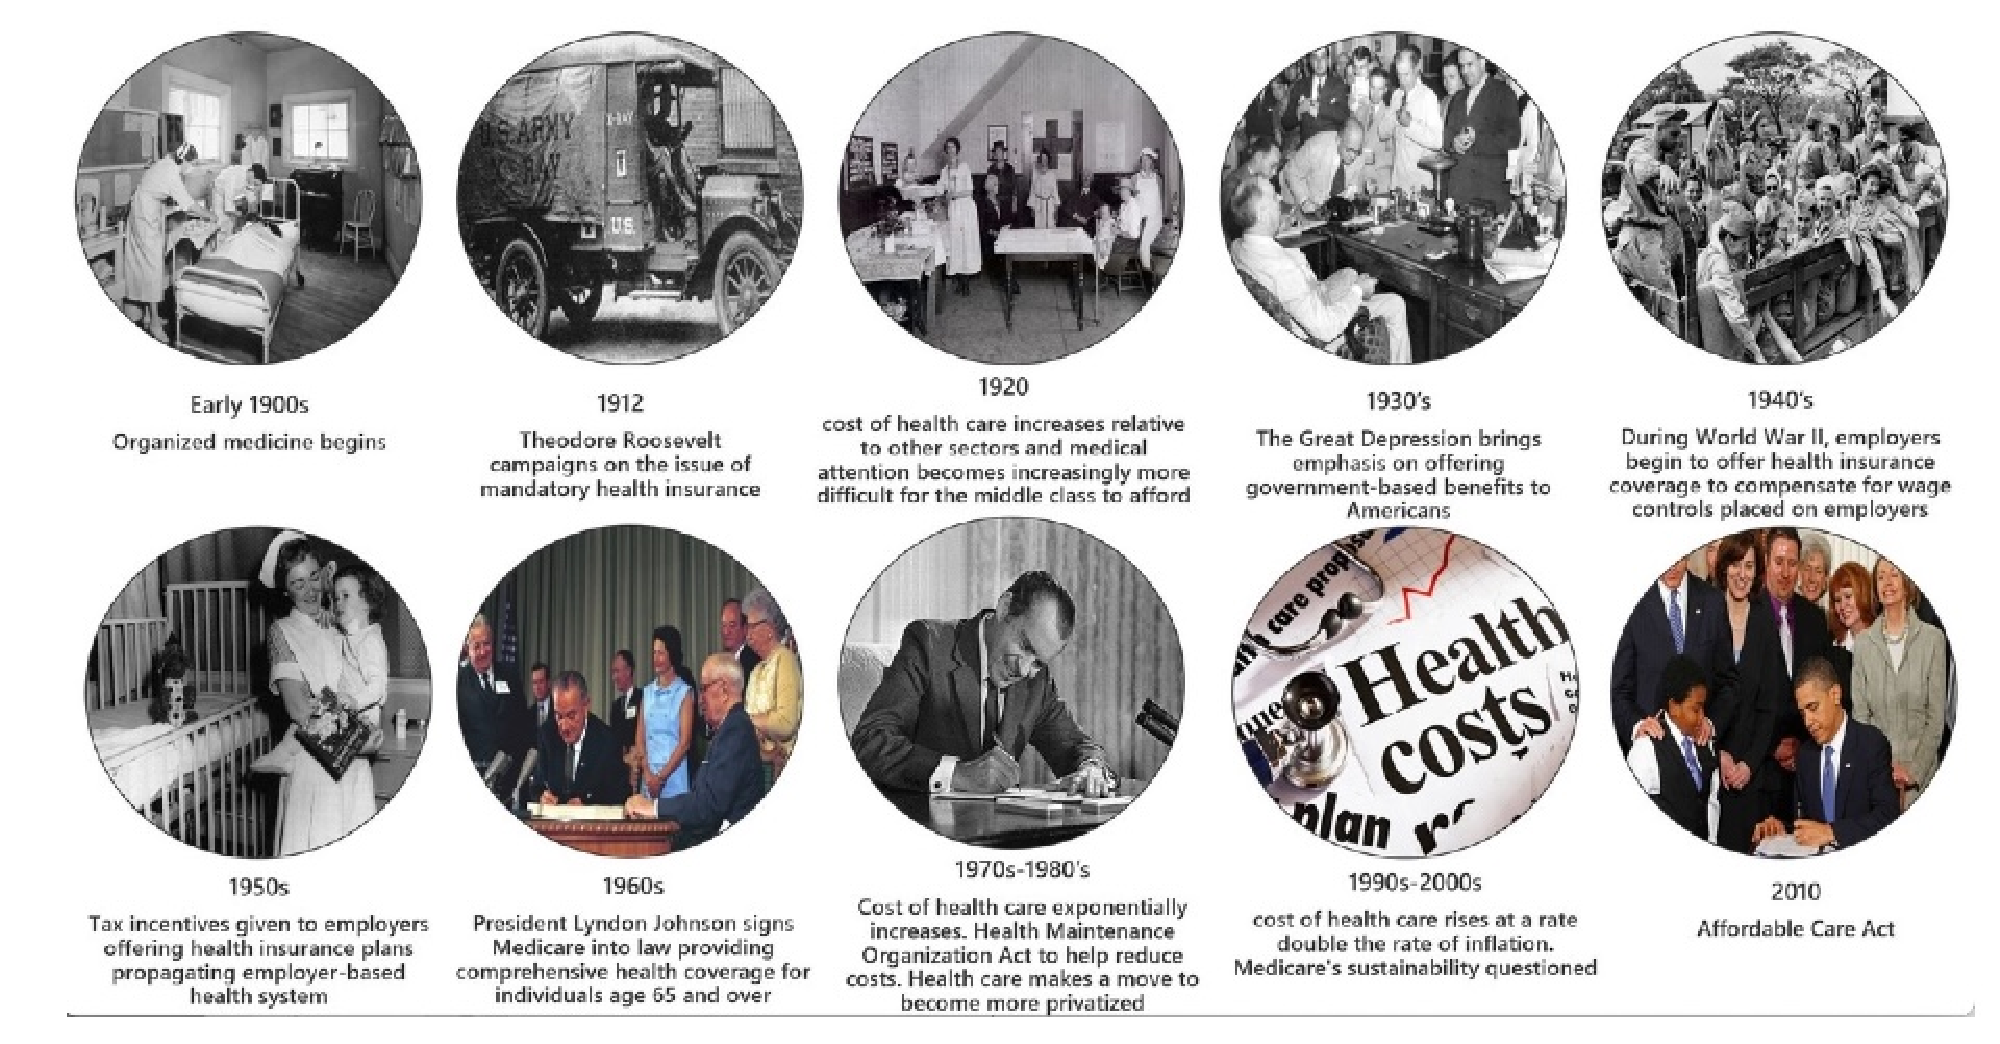
\includegraphics[height=0.9\textheight]{input/history_insurance.pdf}
    \end{center}
\end{frame}
%---------------------------------------------------------------------
\begin{frame}{What about \newbold{public insurance}?}

    \begin{columns}[T]   % T = top alignment
        % ---------------- LEFT COLUMN ----------------
        \begin{column}{0.6\textwidth}
            \begin{itemize}
                \item Social Security Amendments of 1965
                \begin{itemize}
                    \item \newbold{Medicare}: coverage for the elderly.
                    \begin{itemize}
                        \item Part A: hospital care
                        \item Part B: physician fees \& outpatient care
                        \item 1972: expanded to include severely disabled and ESRD
                    \end{itemize}
                    \item \newbold{Medicaid}: coverage for ``nonelderly indigent''.
                    \begin{itemize}
                        \item Means-tested
                        \item Shared federal-state program
                    \end{itemize}
                \end{itemize}
            \end{itemize}
        \end{column}
    
        % ---------------- RIGHT COLUMN ----------------
        \begin{column}{0.4\textwidth}
            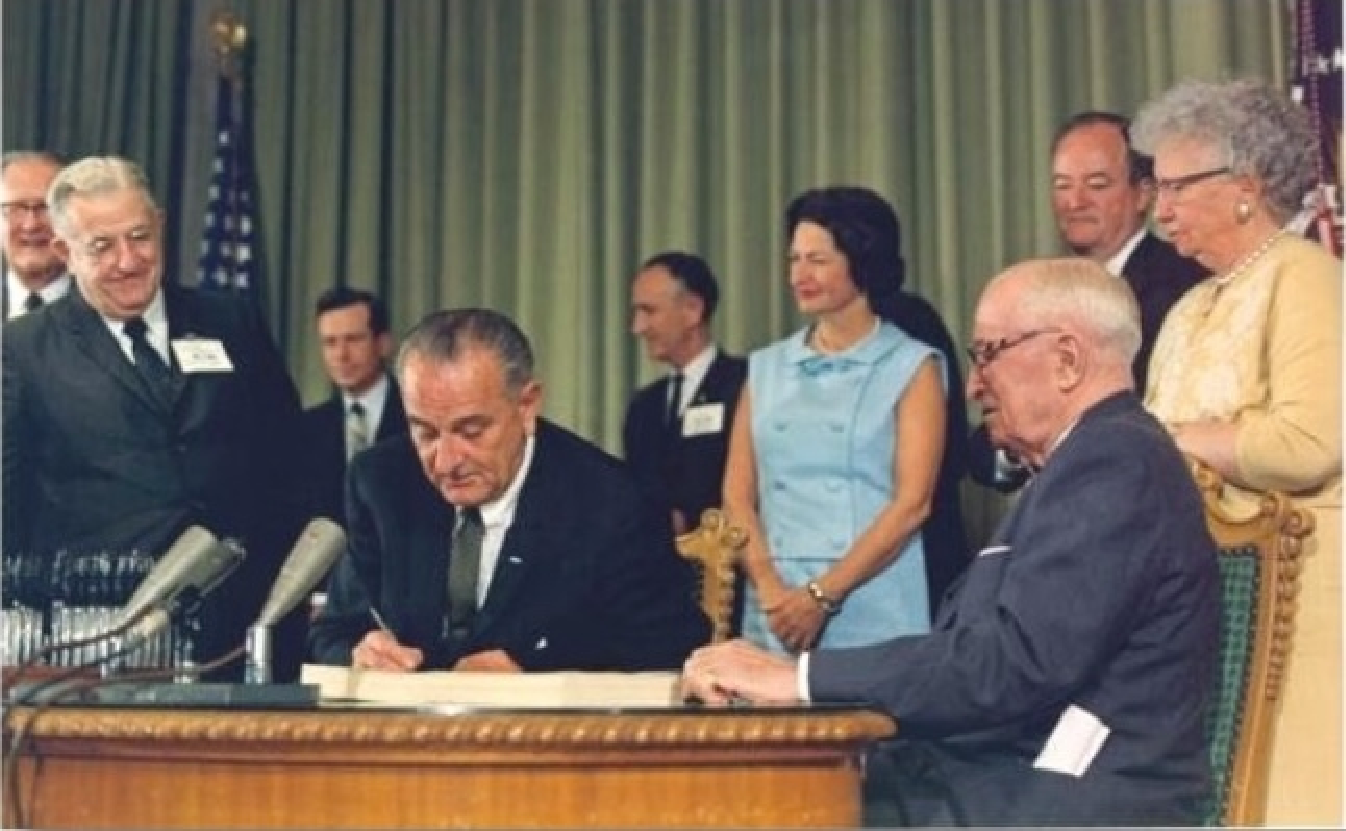
\includegraphics[width=1.1\textwidth]{input/johnson65_Medicare.pdf}
        \end{column}
    \end{columns}

        % \textit{Side note}: How did they get hospitals and physicians onboard?
        %     \begin{itemize}
        %         \item Leveraged existing insurer-provider relationships: paid through private insurers
        %         \item Hospitals paid based on cost: made possible hospital expansions
        %     \end{itemize}
        %     %extremely expensive
\vspace{10mm}
\hbox{\hspace{-8mm} \color{gray} \footnotesize More details in chapter 5 of Emanuel's book (2014)}
% Political history. See chapter 5 of Emanuel's book.
% the ghost of ``socialized medicine'' by AMA
\end{frame}
%---------------------------------------------------------------------
\begin{frame}{What about public insurance? }

\begin{itemize}
        \item The Children's Health Insurance Program (CHIP) 1997
        \vspace{3mm}

        \item Medicare Prescription Drug Improvement and Modernization Act 2003
        \begin{itemize}
            \item Part D: voluntary prescription drug benefit for Medicare eligible
            \item \newbold{Medicare Advantage} (also called part C)
            \begin{itemize}
                \item Really started with Balanced Budget Act 1997
                \item More choice and supplemental coverage (e.g prescription drug, dental, etc.)
            \end{itemize}
        \end{itemize}

    \end{itemize}

\end{frame}
%---------------------------------------------------------------------
% CHIP = public health insurance for children in families that earn too much to qualify for Medicaid but too little to afford private insurance.
% Created in 1997
% Joint federal–state program
% Covers children (and in some states pregnant women)
% Benefits similar to Medicaid but often with small premiums or copays

%Part D: came about because of a growing political and economic crisis over prescription drug access for seniors,
%combined with a deliberate decision to expand public insurance without creating a government-run drug benefit.
% Under George W Bush
%---------------------------------------------------------------------
\begin{frame}{Medicare today}
    \vspace{-7mm}
    \begin{center}
        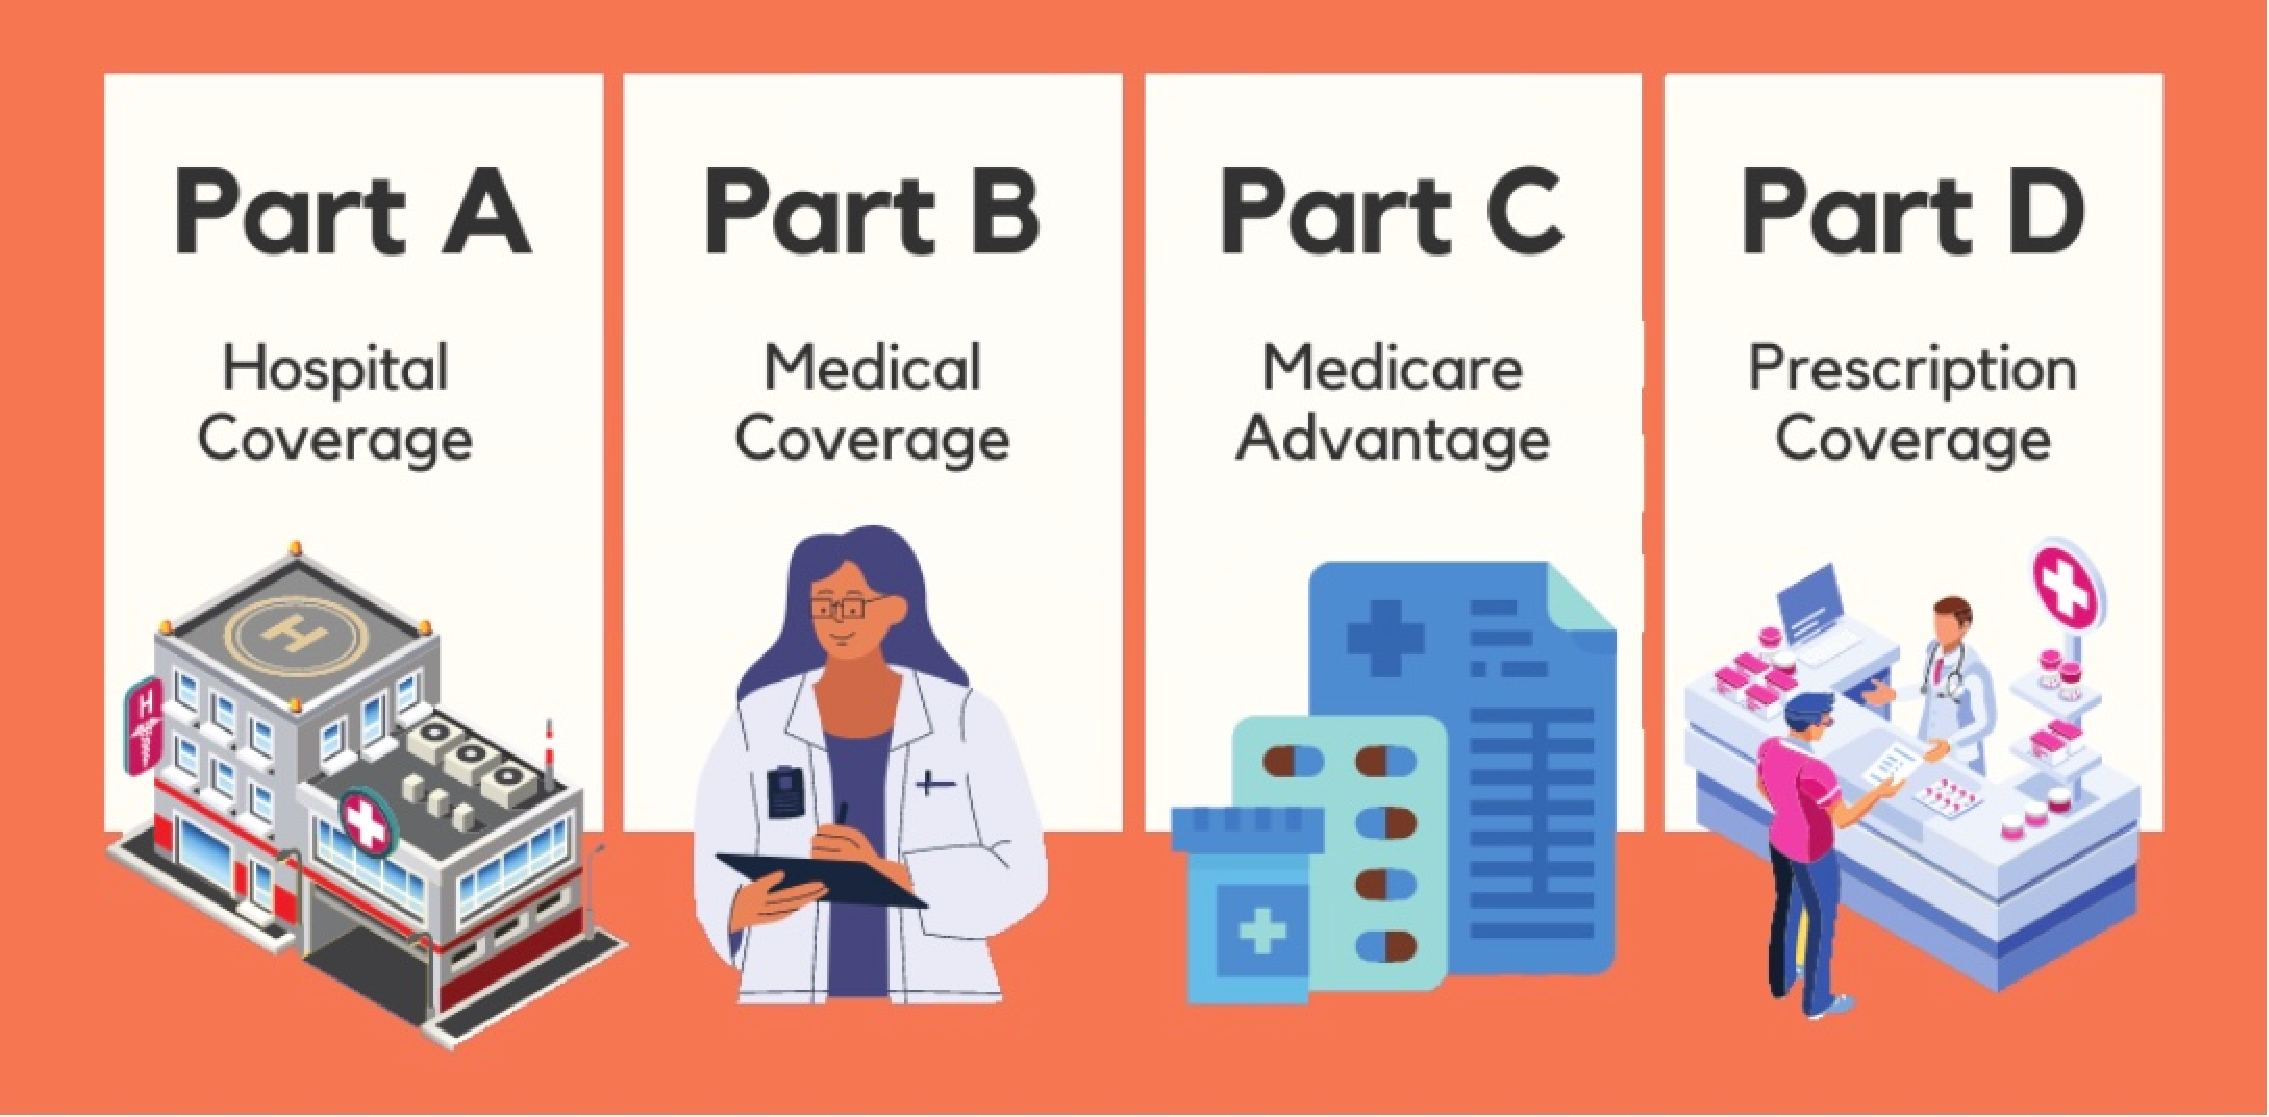
\includegraphics[height=0.85\textheight]{input/Medicare_today.pdf}
    \end{center}
\end{frame}
%---------------------------------------------------------------------

%---------------------------------------------------------------------
\begin{frame}{Why is it important?}
    \begin{center}
        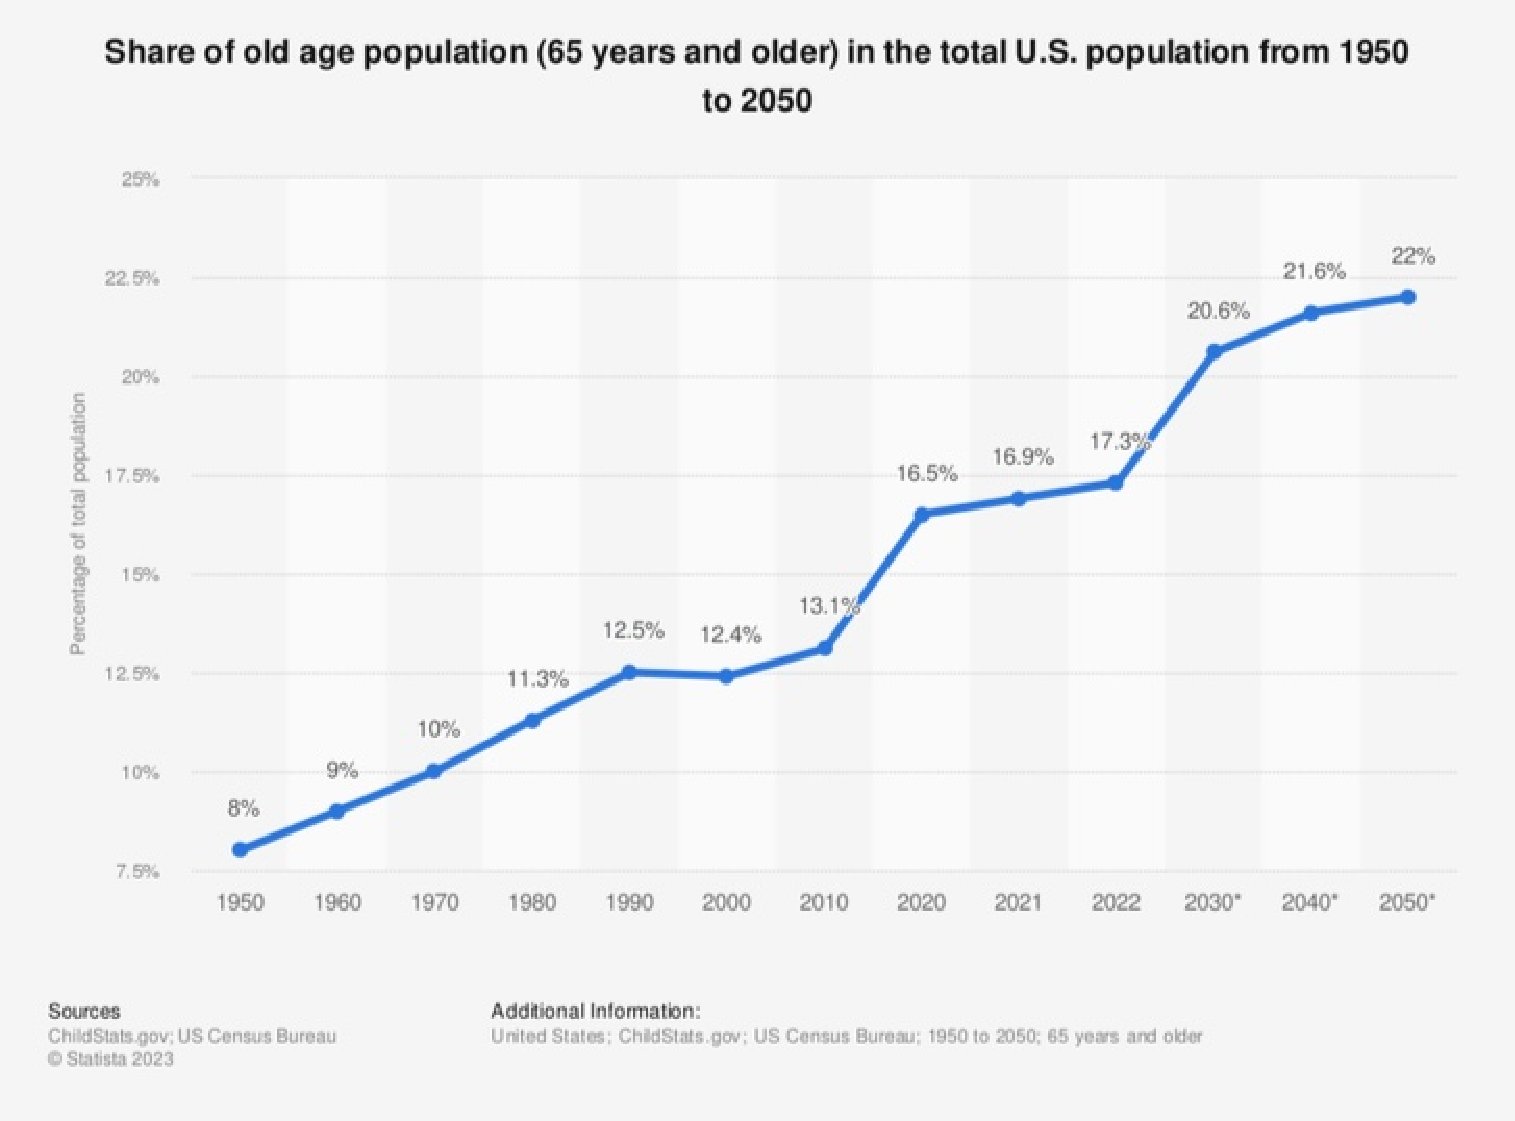
\includegraphics[height=0.9\textheight]{input/share_old.pdf}
    \end{center}
\end{frame}
%---------------------------------------------------------------------

%---------------------------------------------------------------------
\begin{frame}{}
    \begin{center}
        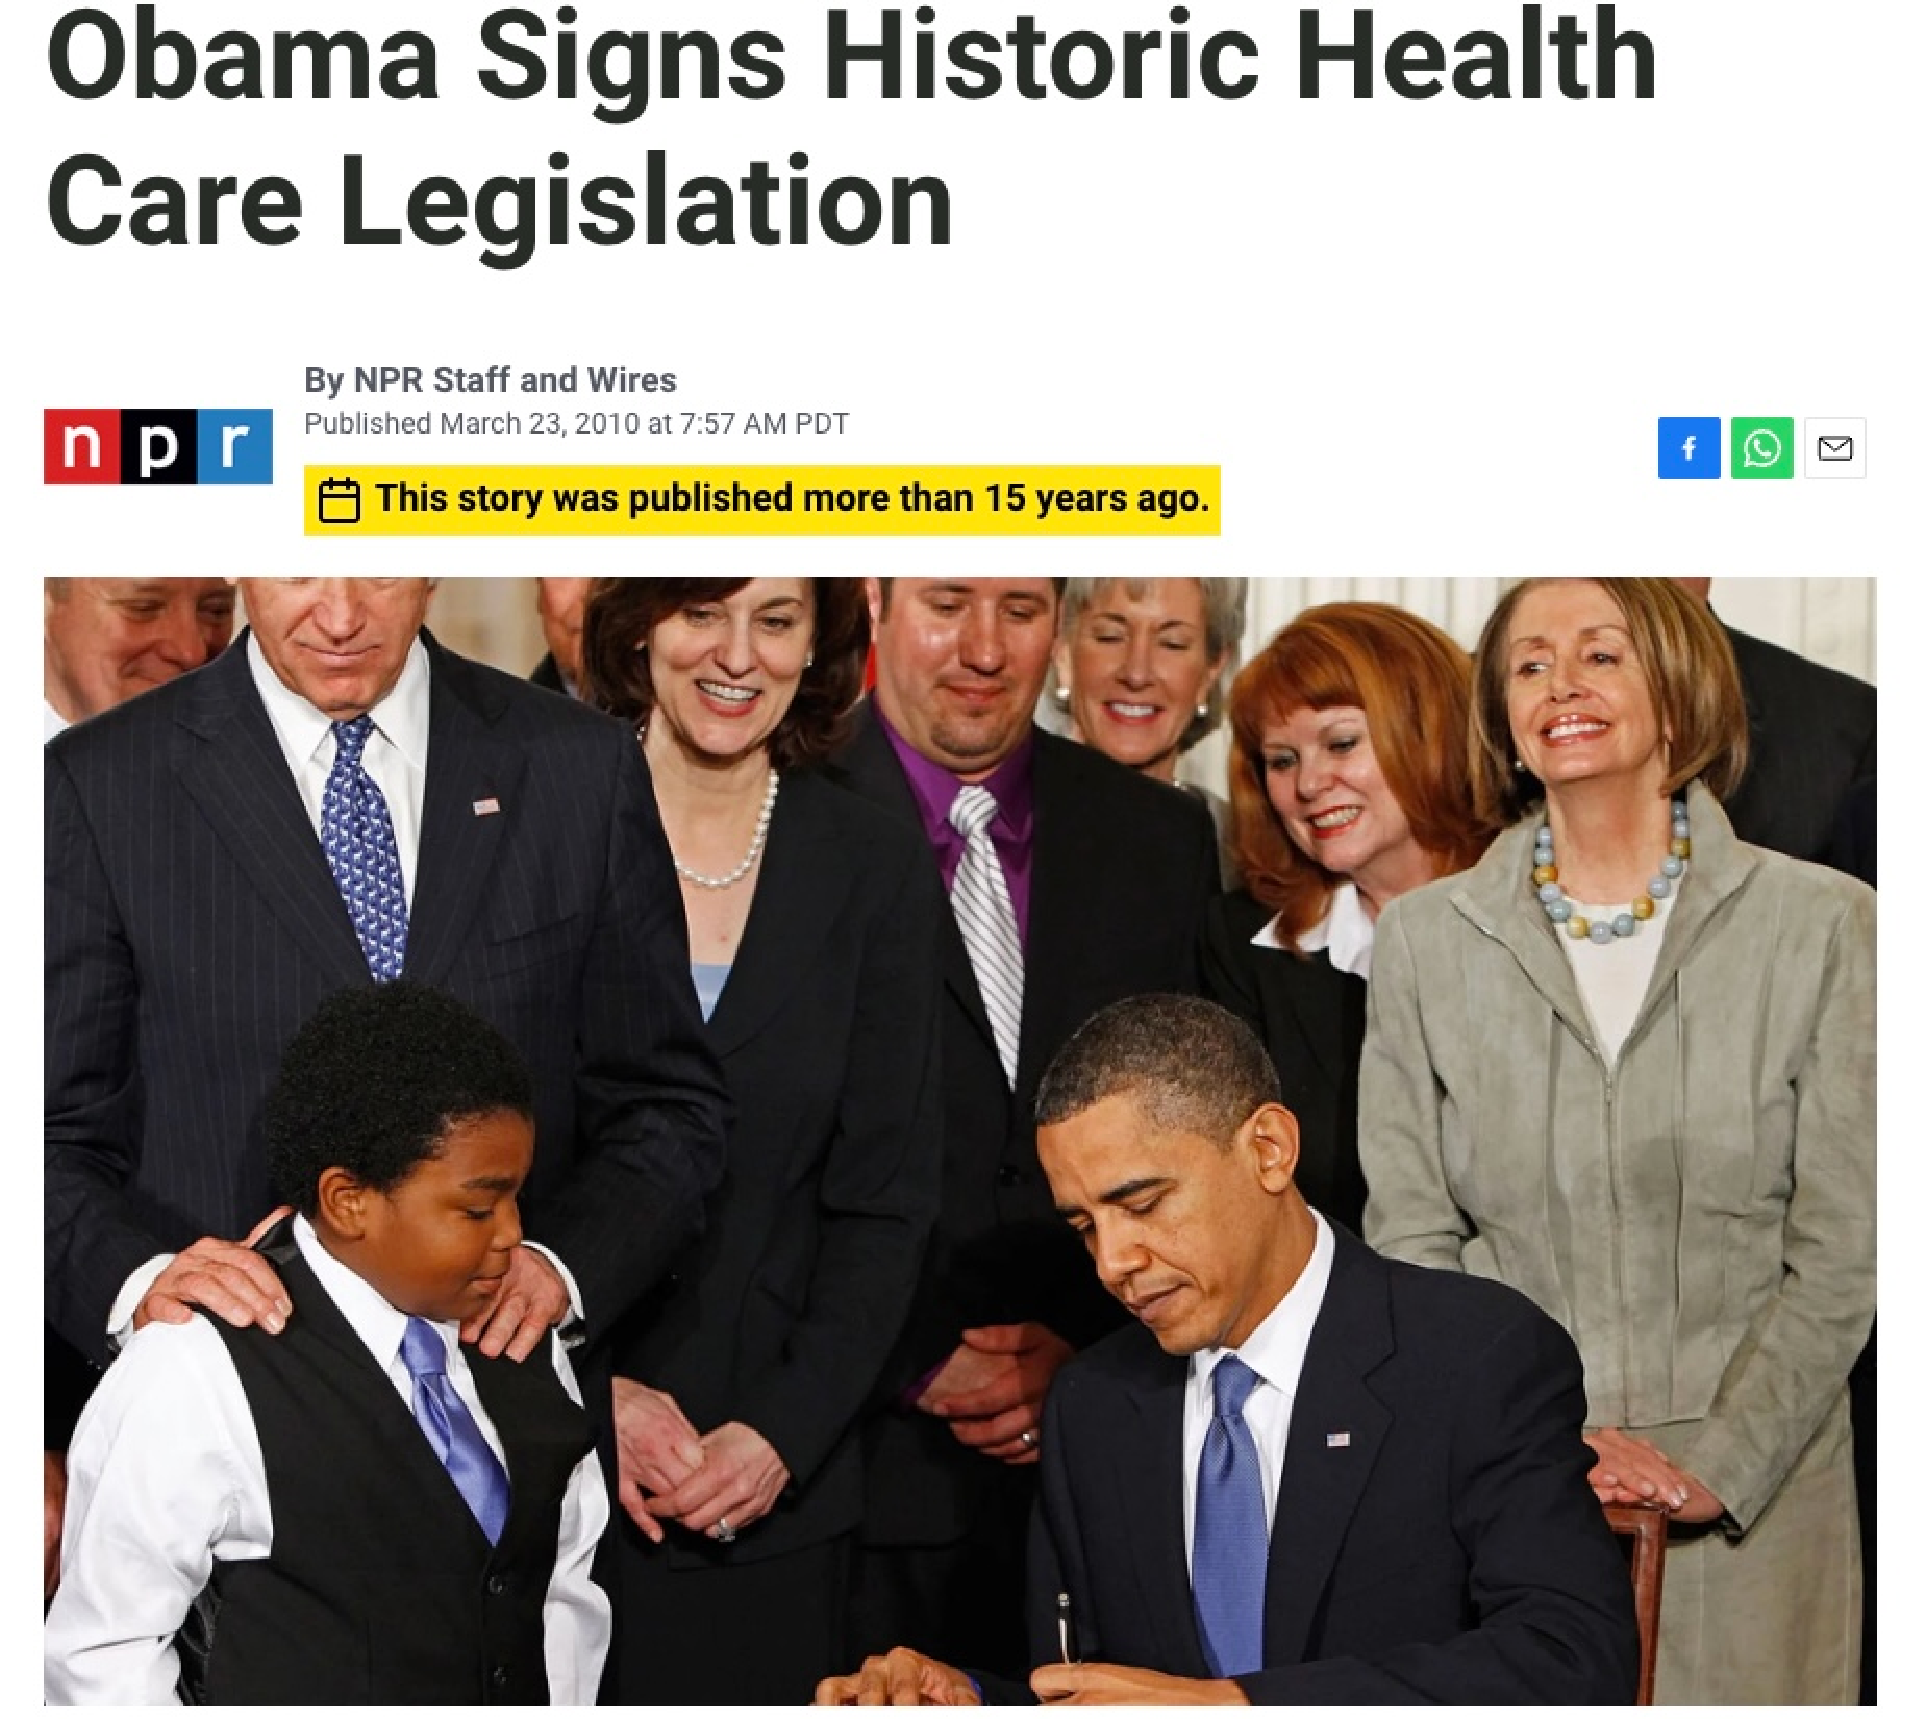
\includegraphics[height=\textheight]{input/obama_aca.pdf}
    \end{center}
\end{frame}
%---------------------------------------------------------------------
\begin{frame}{2010: Affordable Care Act (ACA)}

        \begin{itemize}
            \item The Affordable Care Act (ACA) 2010
            \begin{itemize}
                \item Many dimensions: access, payment, quality incentives, etc.
                \item Access: \newbold{Medicaid expansions}
                    \begin{itemize}
                        \item Increased the threshold
                        \item Expanded benefits
                        \item Increased payments to providers for primary care
                        \item Cost of these expansions borne by federal government
                    \end{itemize}

                    \item Access: \newbold{Health insurance exchanges}
                    \begin{itemize}
                        \item State-based
                        \item Regulated: minimum coverage, quality ratings, etc.
                        \item Subsidized: premium and cost-sharing subsidies
                    \end{itemize}
            \end{itemize}
        \end{itemize}
        \vspace{5mm}
    \hbox{\hspace{-8mm} \color{gray} \footnotesize More details: chapter 8 of Emanuel's book (2014)}
\end{frame}
%---------------------------------------------------------------------

%---------------------------------------------------------------------
\begin{frame}{Rate of uninsurance}
    \vspace{-2mm}
    \begin{center}
        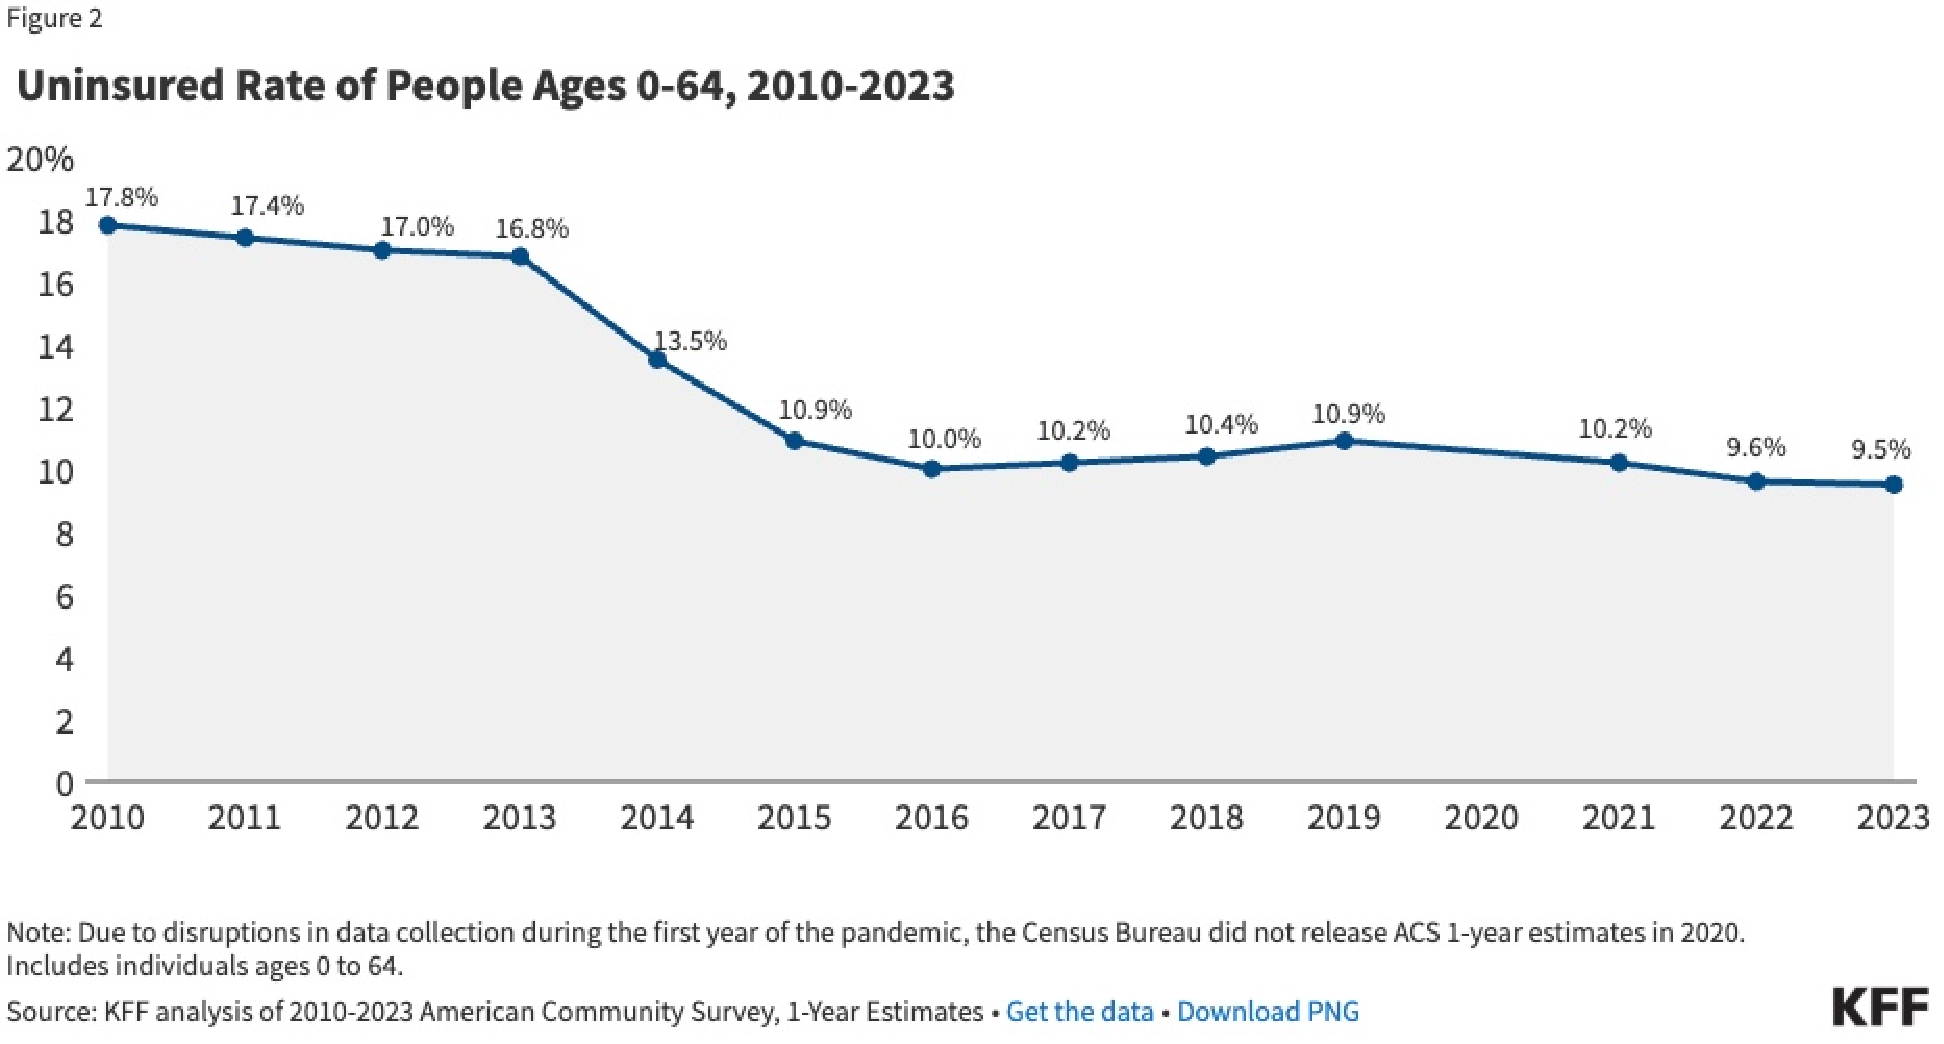
\includegraphics[height=0.8\textheight]{input/KFF_uninsured.pdf}
    \end{center}
    \vspace{-3mm}

    %\only<2>{$\implies$ Who pays for it? \newbold{Mandatory reading 1} for next class {\small (chapter I.3 of Better Health Economics from Gross and Notowidigdo)}}
\end{frame}
%---------------------------------------------------------------------

%---------------------------------------------------------------------
\begin{frame}{}
    \begin{center}
        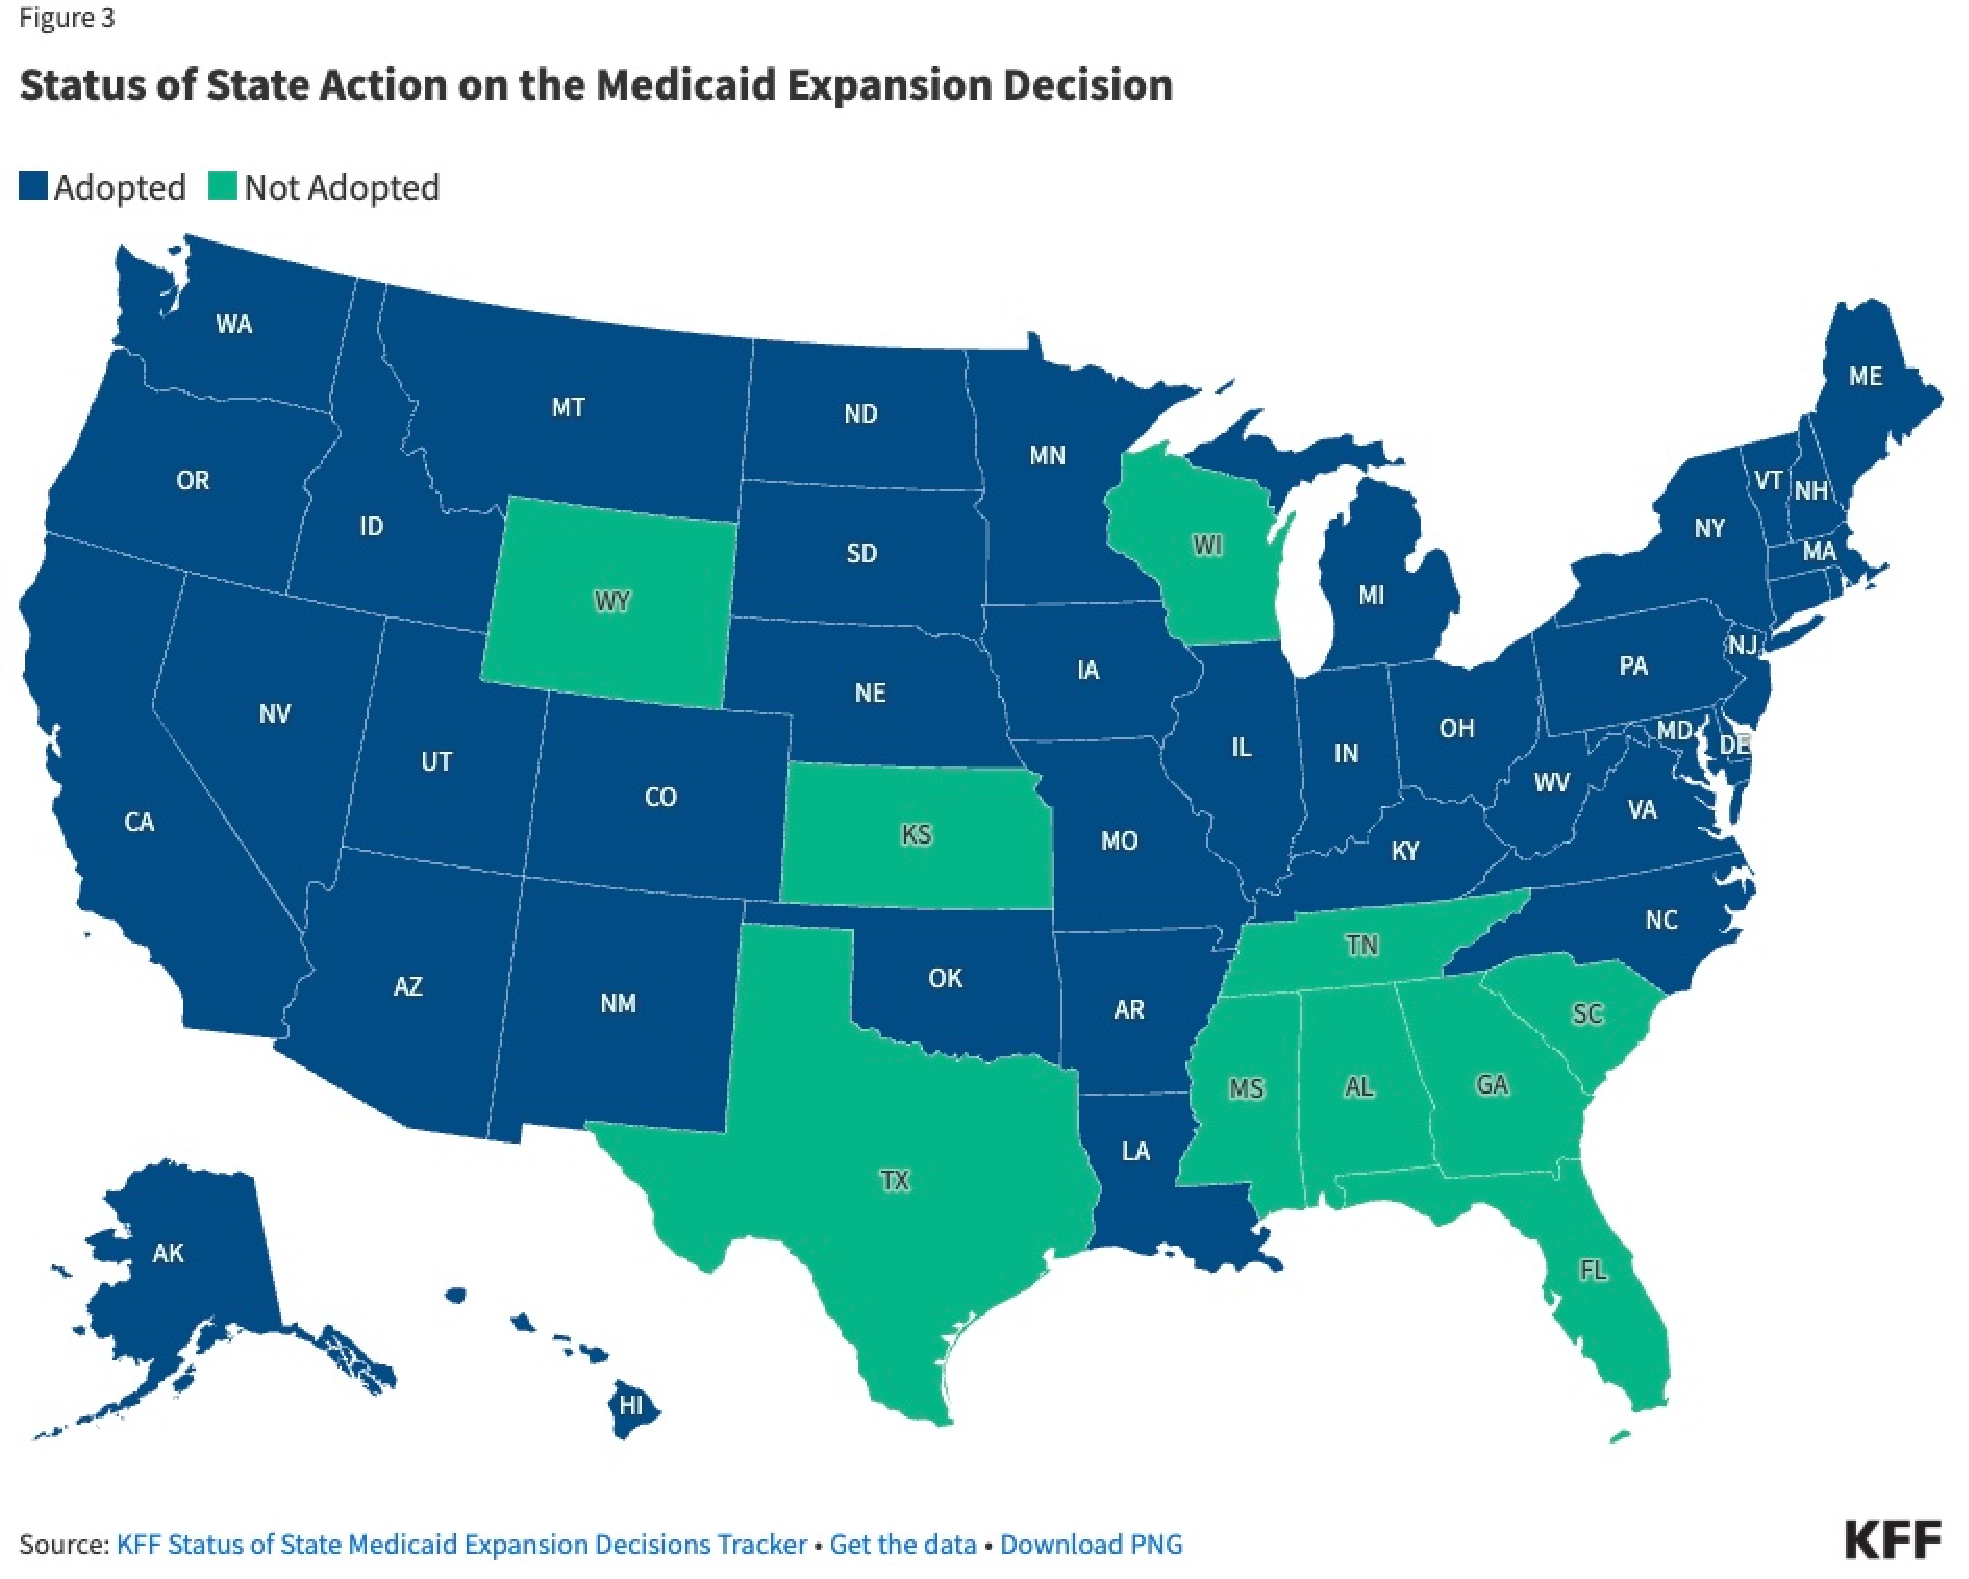
\includegraphics[height=0.95\textheight]{input/KFF_map_ACAexpansionadoption.pdf}
    \end{center}
\end{frame}
%---------------------------------------------------------------------

%---------------------------------------------------------------------
\begin{frame}{}
    \begin{center}
    \Large \textcolor{maroon}{Wrapping up}
    \end{center}

\end{frame}
%---------------------------------------------------------------------
%---------------------------------------------------------------------
\begin{frame}{}
    \vspace{-5mm}
    \begin{center}
        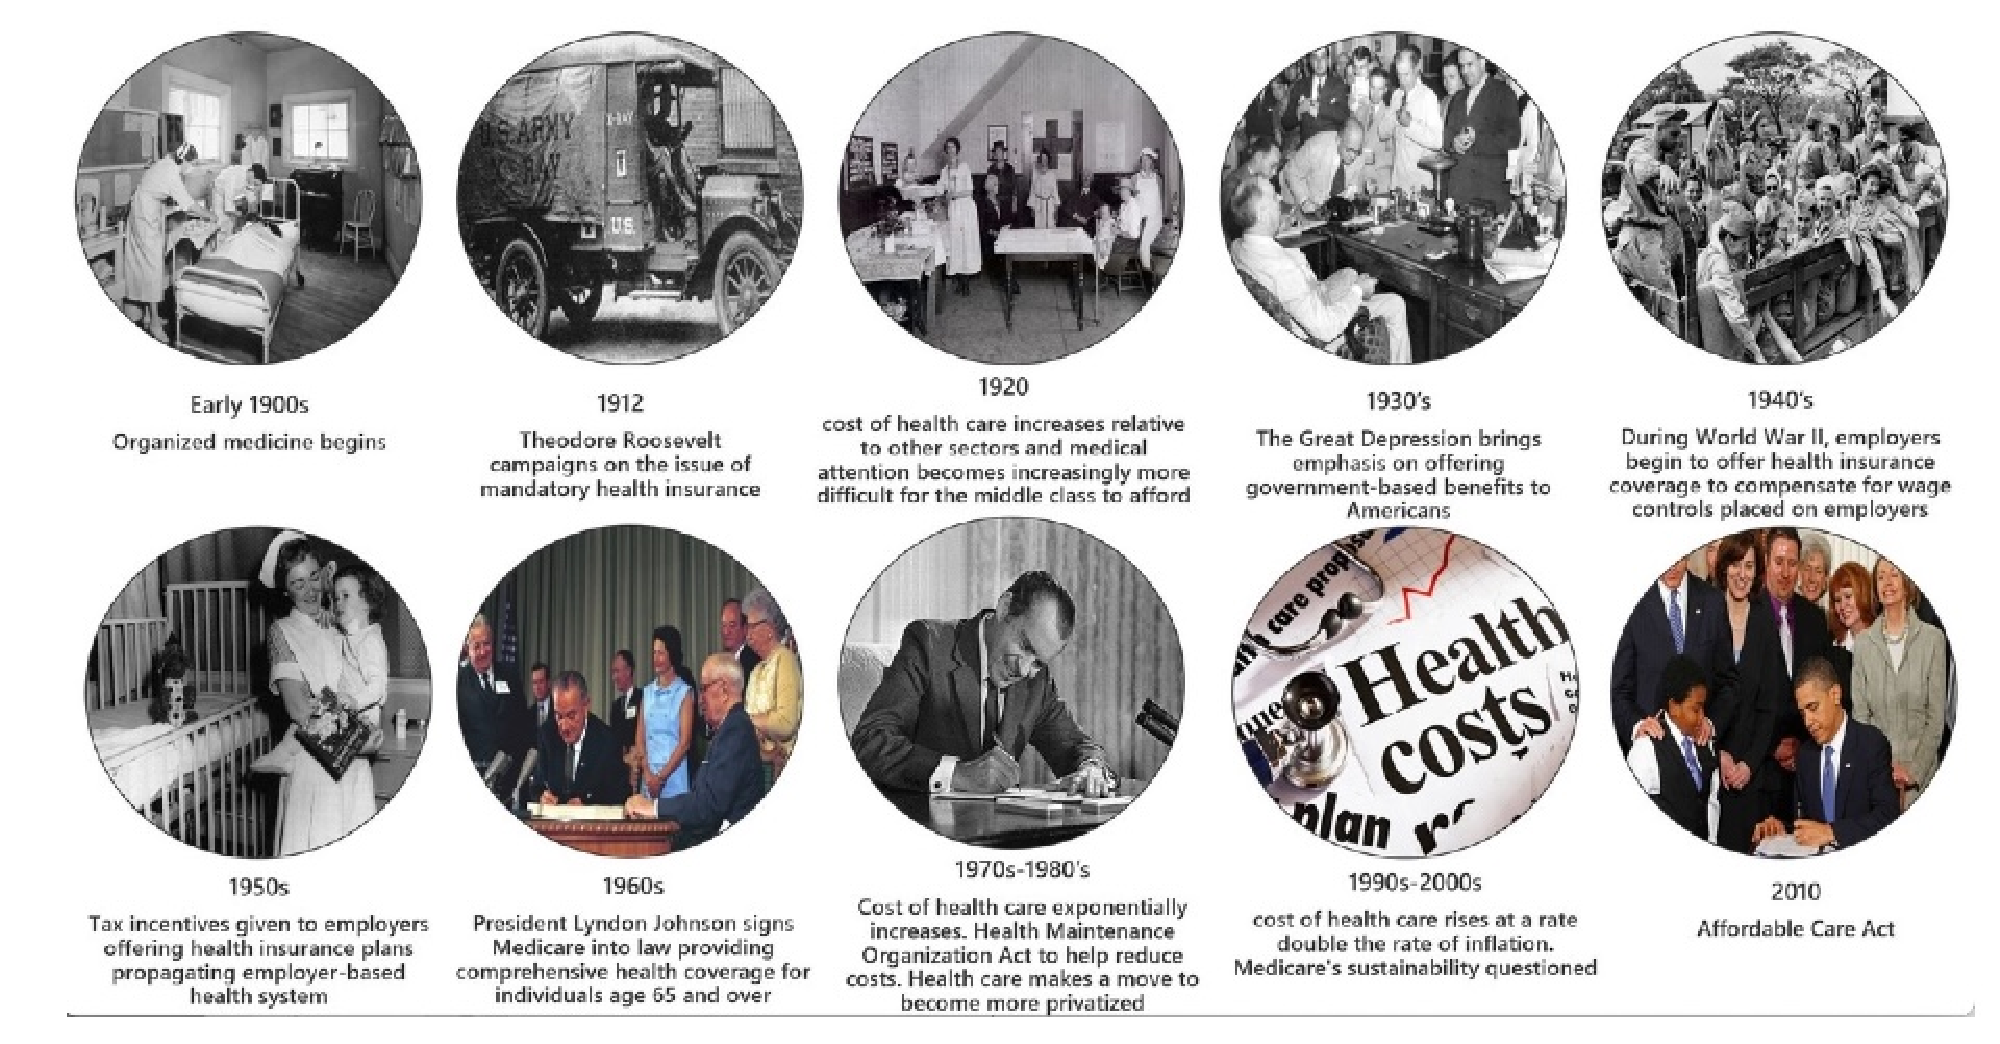
\includegraphics[height=0.9\textheight]{input/history_insurance.pdf}
    \end{center}
\end{frame}
%---------------------------------------------------------------------